\chapter{Theoretical Background}
\label{chapter:background}

In this chapter we give a short survey of the theory of automata and formal languages and introduce the notation for all subsequent chapters.

The material used in this chapter comes from \cite{RozSal97I, HopcroftMotwaniUllman07}, and the free encyclopedia Wikipedia (\url{http://en.wikipedia.org/}). The overall structure of this chapter and some formulations are taken from \cite{C10Diploma}.

In Section \ref{section:words-and-languages} (according to \cite{MaSa1997formal}) we give the reader some preliminary views about the very basics of the formal language theory, about words and languages. In Section \ref{section:regular-languages} (using \cite{Sh1997regular}) we focus on regular languages. We describe several types of finite automata, introduce regular expression, and mention some standard properties of regular languages. In Section \ref{section:context-free-languages} we investigate context-free languages, grammars, and their normal forms (we follow \cite{AuBeBo1997context-free}). We also define pushdown automata as a device for accepting context-free languages, and mention some of the most important subfamilies of this family. The last Section \ref{section:chomsky-hierarchy} (according to \cite{MaSa1997aspects}) is devoted to Chomsky hierarchy of grammars and languages. We cover some properties  of type $0$ (phrase-structure) and type $1$ (context-sensitive) grammars and languages.

\section{Words and Languages}
\label{section:words-and-languages}

An \index{alphabet}\emph{alphabet} is a finite nonempty set. The elements of an alphabet $\Sigma$ are called \index{letter}\emph{letters} or \index{symbol}\emph{symbols}. A \index{word}\emph{word} or \index{string}\emph{string} over an alphabet $\Sigma$ is a finite sequence consisting of zero or more letters of $\Sigma$, whereby the same letter may occur several times. The sequence of zero letters is called the \index{word!empty} \emph{empty word}, written $\lambda$. The set of all words (all nonempty words, respectively) over an alphabet $\Sigma$ is denoted by $\Sigma^*$ ($\Sigma^+$, respectively). If $x$ and $y$ are words over $\Sigma$, then so is their \index{catenation}\emph{catenation} (or \index{concatenation}\emph{concatenation}) $xy$ (or $x \cdot y$), obtained by juxtaposition, that is, writing $x$ and $y$ one after another. Catenation is an associative operation and the empty word $\lambda$ acts as an identity: $w \lambda = \lambda w = w$ holds for all words $w$. Because of the associativity, we may use the notation $w^i$ in the usual way. By definition, $w^0 = \lambda$.

Let $u$ be a word in $\Sigma^*$, say $u = a_1 \ldots a_n$ with $a_i \in \Sigma$. We use $u[i]$ to denote the $i$th letter of $u$, i.e. $u[i] = a_i$. We say that $n$ is the \index{length}\emph{length} of $u$ and we write $|u|=n$. The sets of all words over $\Sigma$ of length $k$, or at most $k$, are denoted by $\Sigma^k$ and $\Sigma^{\le k}$, respectively. By $|u|_a$, for $a \in \Sigma$, we denote the total number of occurrences of the letter $a$ in $u$. The \index{reversal}\emph{reversal} \index{mirror image}(\emph{mirror image}) of $u$, denoted $u^R$, is the word $a_n \ldots a_1$. Finally a \index{factorization}\emph{factorization} of $u$ is any sequence $u_1$, ..., $u_t$ of words such that $u = u_1 \cdots u_t$.

For a pair $u$, $v$ of words we define four relations:

\begin{enumerate}
\item $u$ is a \index{prefix}\emph{prefix} of $v$, if there exists a word $z$ such that $v = uz$,
\item $u$ is a \index{suffix}\emph{suffix} of $v$, if there exists a word $z$ such that $v = zu$, and
\item $u$ is a \index{factor}\emph{factor} (or \index{subword}\emph{subword}) of $v$, if there exist words $z$ and $z'$ such that $v = zuz'$.
\item $u$ is a \index{subword!scattered}\emph{scattered subword} of $v$, if $v$ as a sequence of letters contains $u$ as a subsequence, i.e. there exist words $z_1, \ldots, z_t$ and $y_0, \ldots, y_t$ such that $u = z_1 \ldots z_t$ and $v = y_0 z_1 y_1 \ldots z_t y_t$.
\end{enumerate}

Observe that $u$ itself and $\lambda$ are subwords, prefixes and suffixes of $u$. Other subwords, prefixes and suffixes are called \emph{nontrivial}.

\index{$\Pref_k(u)$}$\Pref_k(u)$ denotes either the (nontrivial) \index{prefix}prefix of length $k$ of the word $u$ in case $|u|>k$, or the whole word $u$ in case $|u|\le k$. Similarly, \index{$\Suff_k(u)$}$\Suff_k(u)$ denotes either the (nontrivial) \index{suffix}suffix of length $k$ of the word $u$ in case $|u|>k$, or the whole word $u$ in case $|u|\le k$. The set of all subwords of length $k$ of $u$ that occur in $u$ in a position other than the prefix or suffix is denoted \index{$\Int_k(u)$}$\Int_k(u)$ \index{interior words}(interior words).

The \index{shuffle}\emph{shuffle} operation between words, denoted $\shuffle$, is defined recursively by $$(au \shuffle bv) = a(u \shuffle bv) \cup b(au \shuffle v),$$ and $$(u \shuffle \lambda) = (\lambda \shuffle u) = \{u\},$$ where $u, v \in \Sigma^*$ and $a, b \in \Sigma$. Obviously, $$(u \shuffle v) = \{x_1 y_1 \ldots x_n y_n \mid u = x_1 \ldots x_n, v = y_1 \ldots y_n, n \ge 1\}.$$

We now proceed from words to languages. Subsets, finite or infinite, of $\Sigma^*$ are referred to as (\emph{formal}) \index{language}\emph{languages} over $\Sigma$. Thus $L_1 = \{\lambda, 0, 111, 1001\}$ and $L_2 = \{0^p \mid p \ \text{is a prime}\}$ are languages over the \index{alphabet!binary}\emph{binary alphabet} $\{0, 1\}$. A \index{language!finite}finite language can always, at least in principle, be defined as $L_1$ above: by listing all of its words. Such a procedure is not possible for \index{language!infinite}infinite languages. Some finitary specification other than simple listing is needed to define an infinite language. 

In formal language theory in general, there are two major types of mechanisms for defining languages: \index{acceptor}\emph{acceptors} and \index{generator}\emph{generators}. Acceptors are usually defined in terms of \index{automaton}\emph{automata}, which work as follows: they are given an input word and after some processing they either accept or reject this input word. For instance, the so-called \index{finite automaton}\emph{finite automata} consist of a finite set of internal states and a set of rules that govern the change of the current state when reading a given input symbol. The finite automaton reads a given input word from left to right starting in a specific \index{state!starting}\emph{starting state}. After reading the input word it accepts only if it ends in one of its \index{state!accepting}\emph{accepting states}, otherwise it rejects. Finite automata recognize the family of \index{language!regular}\emph{regular languages}, which plays a central role in the whole formal language theory (see Section \ref{section:regular-languages}).

Generators, on the other hand, usually generate the language using some finite set of rules. Typically they are defined in terms of grammars. One of the most famous is the classical \index{Chomsky hierarchy}\emph{Chomsky hierarchy} of grammars (and corresponding languages), which consists of \index{grammar!phrase-structure}\emph{phrase-structure}, \index{grammar!context-sensitive}\emph{context-sensitive}, \index{grammar!context-free}\emph{context-free}, and \index{grammar!regular}\emph{regular} grammars. They are also called type $0$, type $1$, type $2$, and type $3$ grammars, respectively (see Section \ref{section:context-free-languages} and \ref{section:chomsky-hierarchy}).

Regarding languages as sets, we may define the \index{operation!Boolean}\emph{Boolean} operations of \index{union}\emph{union}, \index{intersection}\emph{intersection} and \index{complementation}\emph{complementation} in the usual fashion. The operation of \emph{catenation} (or \index{concatenation}\emph{concatenation}) is extended to concern languages in the natural way: $$L_1 L_2 = \{w_1 w_2 \mid w_1 \in L_1 \ \text{and} \ w_2 \in L_2\}.$$

The notation $L^i$ is extended to concern languages, now $L^0 = \{\lambda\}$. The \index{concatenation!closure}\emph{catenation closure} or \index{Kleene star} \emph{Kleene star} \index{Kleene plus}(\emph{Kleene plus}, respectively) of a language $L$, in symbols $L^*$ ($L^+$, respectively) is defined to be the union of all nonnegative powers of $L$ (of all positive powers of $L$, respectively). Observe that this definition is in accordance with our earlier notations $\Sigma^*$ and $\Sigma^+$ if we understand $\Sigma$ as the finite language whose words are the singleton letters. The \index{language!reversal}\emph{reversal} \index{language!mirror image}(\emph{mirror image}) of a language $L$, denoted $L^R$, is the set $$L^R = \{w^R \mid w \in L\}.$$

For each $x \in \Sigma^*$, the \index{left-derivate}\emph{left-derivate} of $L$ with respect to $x \in \Sigma^*$ is the set $$\delta_x(L) = x \backslash L = \{y \in \Sigma^* \mid xy \in L\},$$ and for a language $L_0 \subseteq \Sigma^*$, the \index{left-quotient}\emph{left-quotient} of $L$ by $L_0$ is the set $$L_0 \backslash L = \bigcup_{x \in L_0} x \backslash L = \{y \in \Sigma^* \mid xy \in L, x \in L_0\}.$$ Similarly, the \index{right-derivate}\emph{right-derivate} of $L$ with respect to $x \in \Sigma^*$ is the set $$\delta^x(L) = L / x = \{y \in \Sigma^* \mid yx \in L\},$$ and the \index{right-quotient}\emph{right-quotient} of $L$ by a language $L_0 \subseteq \Sigma^*$ is $$L / L_0 = \bigcup_{x \in L_0} L / x = \{y \in \Sigma^* \mid yx \in L, x \in L_0\}.$$

It is clear by the above definition that $$(L_1 \backslash L) \cup (L_2 \backslash L) = (L_1 \cup L_2) \backslash L$$ for any $L_1, L_2 \subseteq \Sigma^*$. Similar equality holds for right-quotient of languages.

Also the \index{shuffle}shuffle operation is extended in the natural to languages:
$$(L_1 \shuffle L_2) = \bigcup_{u \in L_1, v \in L_2}(u \shuffle v).$$

The operations of union, catenation, and Kleene star are referred as \index{operation!regular}\emph{regular} operations. A language $L$ over $\Sigma$ is termed \index{language!regular}\emph{regular} if $L$ can be obtained from the \index{language!atomic}``atomic'' languages $\emptyset$ (the \index{language!empty} empty language) and $\{a\}$, where $a$ is a letter of $\Sigma$, by applying regular operations finitely many times. By applying union and catenation, we obviously get all \index{language!finite}finite languages \index{$\Fin$}($\Fin$). The star operation is needed to produce \index{language!infinite}infinite languages. In fact, for any $k$, there are regular languages that cannot be represented with fewer than $k$ nested star operations. When we speak of the \emph{family} of regular languages, we mean all languages that are regular over some $\Sigma$, that is, the alphabet may vary from language to language. The family of regular languages has many desirable formal properties. It is closed under most of the usual operations for languages, in particular, under all Boolean operations.

A language $L$ over $\Sigma$ is \index{language!star-free}\emph{star-free} if $L$ can be obtained from the atomic languages $\{a\}$, where $a \in \Sigma$, by applying \index{operation!Boolean}Boolean operations (complement is taken with respect to $\Sigma^*$) and catenation finitely many times. Apparently every star-free language is regular.

We say that a language $L$ is \index{language!noncounting}\emph{noncounting} if there is an integer $n$ such that, for all words $x$, $y$, $z$, $$x y^n z \in L \Leftrightarrow x y^{n+1} z \in L.$$

It can be proved that every star-free language is noncounting. The converse holds in the form: every regular noncounting language is star-free.

A special subclass of star-free languages which has attracted much attention is the \index{language!locally testable}\emph{locally testable languages}. Informally, for a locally testable language $L$, one can decide whether a word $w$ is in $L$ by looking at all subwords of $w$ of a previously given length $k$. Formally, a language $L \subseteq \Sigma^*$ is said to be \index{language!$k$-testable}\emph{$k$-testable} if, for any words $x, y \in \Sigma^*$, $|x|, |y| \ge k$, the conditions \index{$\Pref_k(u)$}$\Pref_k(x) = \Pref_k(y)$, \index{$\Suff_k(u)$}$\Suff_k(x) = \Suff_k(y)$, and \index{$\Int_k(u)$}$\Int_k(x) = \Int_k(y)$ imply that $x \in L \Leftrightarrow y \in L$. A language is said to be \index{language!locally testable}\emph{locally testable} if it is $k$-testable for some integer $k \ge 1$.

Let $\Sigma$ and $\Gamma$ be two finite alphabets. A mapping $h: \Sigma^* \to \Gamma^*$ is called a \index{morphism}\emph{morphism} if $h(xy) = h(x) h(y)$ for all $x, y \in \Sigma^*$. In particular, $h(\lambda) = \lambda$.

For a set $S$, let \index{$2^S$}$2^S$ (or \index{$\mathcal{P}(S)$}$\mathcal{P}(S)$) denote the \index{power set}\emph{power set} of $S$, i.e. the collection of all subsets of $S$. A mapping $\phi: \Sigma^* \to 2^{\Gamma^*}$ is  called a \index{substitution}\emph{substitution} if $\phi(\lambda) = \{\lambda\}$ and $\phi(xy) = \phi(x) \phi(y)$ for all $x, y \in \Sigma^*$.

Clearly, a morphism is a special kind of substitution where each word is associated with a singleton set. Morphisms and substitutions are usually defined by specifying only the image of each letter in $\Sigma$ under the mapping. We extend the definitions of $h$ and $\phi$, respectively, to define $$h(L) = \{h(w) \mid w \in L\}$$ and $$\phi(L) = \bigcup_{w \in L}\phi(w)$$ for $L \subseteq \Sigma^*$.

A morphism $h: \Sigma^* \to \Gamma^*$ is said to be \index{morphism!$\lambda$-free}$\lambda$-free if $h(a) \neq \lambda$ for all $a \in \Sigma$. A substitution $\phi: \Sigma^* \to 2^{\Gamma^*}$ is said to be \index{substitution!$\lambda$-free}$\lambda$-free if $\lambda \notin \phi(a)$ for all $a \in \Sigma$. And $\phi$ is called a \index{substitution!finite} \emph{finite substitution} if, for each $a \in \Sigma$, $\phi(a)$ is a finite subset of $\Gamma^*$. Similarly, $\phi$ is called a \index{substitution!regular} \emph{regular substitution} if, for each $a \in \Sigma$, $\phi(a)$ is a regular language over $\Gamma$.

Let $h: \Sigma^* \to \Gamma^*$ be a morphism. The \index{morphism!inverse} \emph{inverse} of the morphism $h$ is a mapping $h^{-1}: \Gamma^* \to 2^{\Sigma^*}$ defined by, for each $y \in \Gamma^*$, $$h^{-1}(y) = \{x \in \Sigma^* \mid h(x) = y\}.$$ Similarly, for a substitution $\phi: \Sigma^* \to 2^{\Gamma^*}$, the \index{substitution!inverse}\emph{inverse} of the substitution $\phi$ is a mapping $\phi^{-1}: \Gamma^* \to 2^{\Sigma^*}$ defined by, for each $y \in \Gamma^*$, $$\phi^{-1}(y) = \{x \in \Sigma^* \mid y \in \phi(x)\}.$$

\section{Regular Languages}
\label{section:regular-languages}

Most of the material covered in this Section is taken from Sheng Yu \cite{Sh1997regular}.

In this section we provide a very short survey of some basic notions concerning the family of \index{language!regular}regular languages. This is by no means a comprehensive survey. For a more thorough introduction we refer the reader to \cite{HopcroftMotwaniUllman07}.

For \index{language!regular} regular languages, the natural acceptors are \index{finite automaton}finite automata and the generators are \index{regular expressions}regular expressions and \index{grammar!right-linear}right \index{grammar!left-linear}(left) linear grammars (see Section \ref{subsection:context-free-subfamilies}).

In Section \ref{subsection:finite-automata} we describe several types of finite automata, all of which accept exactly the family of regular languages. In Section \ref{subsection:regular-expressions} we introduce regular expressions and their relationship to finite automata. The last Section \ref{subsection:properties-of-regular-languages} gives some properties of regular languages.

\subsection{Finite Automata}
\label{subsection:finite-automata}

\index{language!regular}Regular languages and \index{finite automaton}finite automata have had a wide range of applications. Their most celebrated application has been lexical analysis in programming language compilation and user-interface translations. Other notable applications include circuit design, text editing, and pattern matching.

A \index{finite automaton}\emph{finite automaton} \index{$\FA$}($\FA$) consists of a finite set of internal states and a set of rules that govern the change of the current state when reading a given input symbol. If the next state is always uniquely determined by the current state and the current input symbol, we say that the automaton is deterministic. Formally, we define a deterministic finite automaton as follows:

A \index{finite automaton!deterministic}\emph{deterministic finite automaton} \index{$\DFA$}($\DFA$) $A$ is a quintuple $(Q, \Sigma, \delta, s, F)$, where:

\begin{enumerate}[]
\item $Q$ is the finite set of \index{state}\emph{states},
\item $\Sigma$ is the \index{alphabet!input}\emph{input alphabet},
\item $\delta: Q \times \Sigma \to Q$ is the \index{transition!function}\emph{state transition function},
\item $s \in Q$ is the \index{state!starting}\emph{starting state}, and
\item $F \subseteq Q$ is the set of \index{state!final}\emph{final states}.
\end{enumerate}

Note that, in general, we do not require the transition function $\delta$ to be total, i.e. to be defined for every pair in $Q \times \Sigma$. If $\delta$ is total, then we call $A$ a \emph{complete} \index{$\DFA$!complete}$\DFA$.

A \index{$\DFA$}$\DFA$ such that every state is reachable from the starting state and reaches a final state is called a \index{$\DFA$!reduced}\emph{reduced} $\DFA$. A reduced $\DFA$ may not be a complete $\DFA$.

A \index{configuration}\emph{configuration} of $A = (Q, \Sigma, \delta, s, F)$ is a word in $Q \Sigma^*$, i.e. a state $q \in Q$ followed by a word $x \in \Sigma^*$ where $q$ is the current state of $A$ and $x$ is the remaining part of the input. The \index{configuration!starting}\emph{starting configuration} of $A$ for an input word $x \in \Sigma^*$ is $sx$.  \index{configuration!accepting}\emph{Accepting configuration} are defined to be elements of $F$ (followed by the empty word $\lambda$).

A \index{computation!step}computation step of $A$ is a \index{transition}transition from a configuration $\alpha$ to a configuration $\beta$, denoted by $\alpha \vdash_A \beta$, where $\vdash_A$ is a binary relation on the set of configurations of $A$. The relation $\vdash_A$ is defined by: for $px, qy \in Q \Sigma^*$, $px \vdash_A qy$ if $x = ay$ for some $a \in \Sigma$ and $\delta(p, a) = q$. We use $\vdash$ instead of $\vdash_A$ if there is no confusion. The transitive closure and the reflexive and transitive closure of $\vdash$ are denoted $\vdash^+$ and $\vdash^*$, respectively.

The language accepted by a \index{$\DFA$}$\DFA$ $A = (Q, \Sigma, \delta, s, F)$, denoted $L(A)$, is defined as follows: $$L(A) = \{w \mid sw \vdash^* f \ \text{for some} \ f \in F\}.$$

For convenience, we define the extension of $\delta$, $\delta^*: Q \times \Sigma^* \to Q$, inductively as follows. We set $\delta^*(q, \lambda) = q$ and $\delta^*(q, xa) = \delta(\delta^*(q, x), a)$, for $q \in Q$, $a \in \Sigma$. Then we can also write: $$L(A) = \{w \mid \delta^*(s, w) = f \ \text{for some} \ f \in F\}.$$

\index{finite automaton!nondeterministic}Nondeterministic finite automata \index{$\NFA$}($\NFA$) are a generalization of \index{$\DFA$}$\DFA$ where, for a given state and an input symbol, the number of possible transitions can be greater than one. Formally, a \index{finite automaton!nondeterministic} \emph{nondeterministic finite automaton} $A$ is a quintuple $(Q, \Sigma, \delta, s, F)$ where $Q$, $\Sigma$, $s$, and $F$ are defined exactly the same way as for a \index{$\DFA$}$\DFA$, and $\delta: Q \times \Sigma \to 2^Q$ is the \index{transition!function}transition function.

The \index{computation!relation}computation relation $\vdash_A: Q \Sigma^* \times Q \Sigma^*$ of an \index{$\NFA$}$\NFA$ $A$ is defined by setting $px \vdash_A qy$ if $x = ay$ and $q \in \delta(p, a)$, for $p, q \in Q$, $x, y \in \Sigma^*$, and $a \in \Sigma$. The language accepted by $A$ is defined in the same way as for \index{$\DFA$}$\DFA$.

\index{$\NFA$}$\NFA$ can be further generalized to have state transitions without reading any input symbol. Such transitions are called \index{transition!$\lambda$-transition} $\lambda$-transitions in the following definition.

A \emph{nondeterministic finite automaton with $\lambda$-transitions} \index{$\lambda$-$\NFA$}($\lambda$-$\NFA$) $A$ is a quintuple $(Q, \Sigma, \delta, s, F)$ where $Q$, $\Sigma$, $s$, and $F$ are the same as for an \index{$\NFA$}$\NFA$; and $\delta: Q \times (\Sigma \cup \{\lambda\}) \to 2^Q$ is the transition function.

For a \index{$\lambda$-$\NFA$}$\lambda$-$\NFA$ $A = (Q, \Sigma, \delta, s, F)$, the binary relation $\vdash_A: Q \Sigma^* \times Q \Sigma^*$ is defined by that $px \vdash_A qy$, for $p, q \in Q$ and $x, y \in \Sigma^*$, if $x = ay$ and $q \in \delta(p, a)$ or if $x = y$ and $q \in \delta(p, \lambda)$. The language accepted by $A$ is again defined in the same way as for \index{$\DFA$}$\DFA$.

Let $A = (Q, \Sigma, \delta, s, F)$ be a \index{$\lambda$-$\NFA$}$\lambda$-$\NFA$. The \index{$\lambda$-closure}\emph{$\lambda$-closure} of a state $q \in Q$, denoted by $\lambda \text{-closure}(q)$, is the set of all states that are reachable from $q$ by zero or more $\lambda$-transitions, i.e. $$\lambda \text{-closure}(q) = \{q \in Q \mid q \vdash_A^* p \}.$$

For a \index{$\lambda$-$\NFA$}$\lambda$-$\NFA$ $A = (Q, \Sigma, \delta, s, F)$ let $A' = (Q, \Sigma, \delta', s, F')$ be an \index{$\NFA$}$\NFA$, such that for each $q \in Q$ and $a \in \Sigma$, $$\delta'(p, a) = \delta(p, a) \cup \bigcup_{q \in \lambda \text{-closure}(p)}\delta(q, a)$$ and $$F' = \{ q \in Q \mid \lambda\text{-closure}(q) \cap F \neq \emptyset \}.$$ It can be easily verified that $L(A) = L(A')$.

Another form of generalization of \index{$\NFA$}$\NFA$ is defined in the following.

A \emph{$\NFA$ with nondeterministic starting state} \index{$\NNFA$}($\NNFA$) $A = (Q, \Sigma, \delta, S, F)$ is an \index{$\NFA$}$\NFA$ except that there is a set of \index{state!starting}starting states $S$ rather than exactly one starting state. Thus, for an input word, the \index{computation}computation of $A$ starts from a nondeterministically chosen \index{state!starting}starting state.

It can be shown that for each $\NNFA$ $A$ of $n$ states, we can construct an equivalent \index{$\DFA$}$\DFA$ $A'$ of at most $2^n$ states.

There are also several models of finite automata with output, which include \index{Moore machine}Moore machines, \index{Mealy machine}Mealy machine, and \index{finite transducer}finite transducers.

\subsection{Regular Expressions}
\label{subsection:regular-expressions}

In the previous section we have described various forms of finite automata. These automata can be easily implemented by computer programs. However, finite automata in any of the above mentioned forms are not convenient to be specified manually by users. A succinct and comprehensible expression in sequential form would be better suited than a finite automaton definition. Such expressions are regular expressions which are often used as user interfaces for specifying regular languages.

We define, inductively, a \index{regular expressions}\emph{regular expression} $e$ over an alphabet $\Sigma$ and the language $L(e)$ it denotes as follows:

\begin{enumerate}
\item $e = \emptyset$ is a regular expression denoting the language $L(e) = \emptyset$.
\item $e = \lambda$ is a regular expression denoting the language $L(e) = \{\lambda\}$.
\item $e = a$, $a \in \Sigma$, is a regular expression denoting the language $L(e) = \{a\}$.

Let $e_1$ and $e_2$ be regular expressions and $L(e_1)$ and $L(e_2)$ be the languages they
denote, respectively. Then
\item $e = (e_1 + e_2)$ is a regular expression denoting the language $L(e) = L(e_1) \cup L(e_2)$.
\item $e = (e_1 \cdot e_2)$ is a regular expression denoting the language $L(e) = L(e_1) L(e_2)$.
\item $e = e_1^*$ is a regular expression denoting the language $(L(e_1))^*$.
\end{enumerate}

We assume that $*$ has higher precedence than $\cdot$ and $+$, and $\cdot$ has higher precedence than $+$. A pair of parentheses may be omitted whenever the omission would not cause any confusion. Also, we usually omit the symbol $\cdot$ in regular expressions.

There are three major approaches for transforming regular expressions into finite automata. The first approach is to transform a regular expression into a \index{$\lambda$-$\NFA$} $\lambda$-$\NFA$. This approach is simple and intuitive, but may generate many \index{transition!$\lambda$-transition}$\lambda$-transitions. The second approach transforms a regular expression into an \index{$\NFA$}$\NFA$ without \index{transition!$\lambda$-transition}$\lambda$-transitions. The third and most involved approach is to transform a regular expression directly into an equivalent \index{$\DFA$}$\DFA$.

The converse is also possible, i.e. for a given finite automaton $A$, we can construct a regular expression $e$ such that $e$ denotes the language accepted by $A$. The construction uses \index{finite automaton!extended}\emph{extended finite automata} where a transition between a pair of states is labeled by a regular expression. For a given finite automaton, a so-called \emph{state elimination technique} deletes a state at each step and changes the transitions accordingly. This process continues until the \index{$\FA$}$\FA$ contains only the starting state, a final state, and the transition between them. The regular expression labeling the transition specifies exactly the language accepted by $A$.

\subsection{Properties of Regular Languages}
\label{subsection:properties-of-regular-languages}

There are many ways to show that a language is regular; for example, this can be done by demonstrating that the language is accepted by a finite automaton, specified by a regular expression, or generated by a right-linear grammar. To prove that a language is not regular, the most commonly used tools are the \emph{pumping properties} of \index{language!regular}regular languages, which are usually stated as \index{pumping lemma}``pumping lemmas''. The term ``pumping'' intuitively describes the property that any sufficiently long word of the language has a nonempty subword that can be ``pumped'', i.e. if the subword is replaced by an arbitrary number of copies of the same subword, the resulting word is still in the language.

There are many versions of pumping lemmas for regular languages. The ``standard'' version is a necessary but not sufficient condition for regularity.

\index{pumping lemma!regular language}
\begin{lemma}
Let $L$ be a regular language over $\Sigma$. Then there is a constant $n$, depending on $L$, such that for each $w \in L$ with $|w| \ge n$ there exist $x, y, z \in \Sigma^*$ such that $w = xyz$ and
\begin{enumerate}
\item $|xy| \le n$,
\item $|y| \ge 1$,
\item $x y^t z \in L$ for all $t \ge 0$.
\end{enumerate}
\end{lemma}

The proof is based on the observation that if an $n$-state $\DFA$ reads a word $w$ of length $|w| \ge n$, then it passes through the sequence of $|w| + 1 > n$ states, thus (by the pigeonhole principle) at least two states in this sequence must be equal.

In the following theorem we summarize some selected closure properties of regular languages.

\begin{theorem}
The family of regular languages is closed under the following operations (we assume that $L \subseteq \Sigma^*$):
\begin{enumerate}
\item Boolean operations: union, intersection, complementation,
\item catenation, Kleene star, reversal,
\item left and right-quotient by an arbitrary language,
\item $\text{prefix}(L) = \{x \in \Sigma^* \mid xy \in L, y \in \Sigma^*\}$,
\item $\text{suffix}(L) = \{y \in \Sigma^* \mid xy \in L, x \in \Sigma^*\}$,
\item $\text{infix}(L) = \{y \in \Sigma^* \mid xyz \in L, x,z \in \Sigma^*\}$,
\item morphism, inverse morphism,
\item finite substitution, inverse finite substitution,
\item regular substitution, inverse regular substitution.
\end{enumerate}
\end{theorem}

Finally, we characterize the family of regular languages by a so-called \index{Myhill-Nerode theorem}Myhill-Nerode Theorem. Let $L \subseteq \Sigma^*$ and $x \in \Sigma^*$. The \emph{derivate} of $L$ with respect to $x$, denoted $D_x L$, is $$D_x L = x \backslash L = \{y \in \Sigma^* \mid xy \in L\}.$$

For $L \subseteq \Sigma^*$, we define a relation $\equiv_L \subseteq \Sigma^* \times \Sigma^*$ by $$x \equiv_L y \Leftrightarrow D_x L = D_y L$$ for each pair $x, y \in \Sigma^*$. Clearly, $\equiv_L$ is an equivalence relation. It partitions $\Sigma^*$ into equivalence classes. The number of equivalence classes of $\equiv_L$ is called the \emph{index} of $\equiv_L$. 
%We denote the equivalence class that contains $x$ by $[x]_{\equiv_L}$, i.e. $$[x]_{\equiv_L} = \{y \in \Sigma^* \mid y \equiv_L x\}.$$ Clearly, $x \equiv_L y$ if and only if $[x]_{\equiv_L} = [y]_{\equiv_L}$. We simply write $[x]$ instead of $[x]_{\equiv_L}$ if there is no confusion.
The following \index{Myhill-Nerode theorem}Myhill-Nerode Theorem characterizes the family of regular languages.

\begin{theorem}
A language $L \subseteq \Sigma^*$ is regular if and only if $\equiv_L$ has a finite index.
\end{theorem}

If $L$ is a regular language, then it can be shown that the minimal number of states of a complete $\DFA$ that accepts $L$ is equal to the index of $\equiv_L$.

\section{Context-Free Languages}
\label{section:context-free-languages}

This section is devoted to \index{language!context-free} context-free languages \index{$\CFL$}($\CFL$). Context-free languages and \index{grammar!context-free} grammars were designed  initially to formalize grammatical properties of natural languages. They subsequently appeared to be well adapted to the formal description of the syntax of programming languages. This led to a considerable development of the theory.

We focus on two basic tools: context-free grammars and \index{pushdown automaton} pushdown automata. These are indeed the standard tools to generate and to recognize context-free languages. In Section \ref{subsection:context-free-grammars} we give a short introduction to context-free grammars, followed by the survey of their \index{normal form}normal forms in Section \ref{subsection:context-free-normal-forms}. In Section \ref{subsection:pushdown-machines} we introduce pushdown automata as a basic accepting device for context-free languages. In the last Section \ref{subsection:context-free-subfamilies} we present some subfamilies of context-free languages.

The main source for this Section is Autebert et al. \cite{AuBeBo1997context-free}.

\subsection{Context-Free Grammars}
\label{subsection:context-free-grammars}

A \index{grammar!context-free}\emph{context-free grammar} $G$ is a quadruple $G = (V_N, V_T, S, P)$, where $V_N$ is disjoint from $V_T$ and:

\begin{enumerate}[]
\item $V_N$ is the finite nonempty set of \index{nonterminal}\emph{nonterminals} or \index{variable}\emph{variables},
\item $V_T$ is the finite nonempty set of \index{terminal}\emph{terminals} or \emph{terminal letters},
\item $S \in V_N$ is the distinguished nonterminal called the \index{axiom}\emph{axiom},
\item $P \subseteq V_N \times (V_N \cup V_T)^*$ is the finite set of \index{production}\emph{productions} or \index{derivation rule}\emph{derivation rules}.
\end{enumerate}

Given words $u, v \in (V_N \cup V_T)^*$, we write $u \Rightarrow_G v$ whenever there exist factorizations $u = x X y$, $v = x \alpha y$, with production $(X, \alpha) \in P$. A \index{derivation}\emph{derivation} of length $k \ge 0$ from $u$ to $v$ is a sequence $(u_0, u_1, \ldots, u_k)$ of words in $(V_N \cup V_T)^*$ such that $u_{i-1} \Rightarrow_G u_i$ for $i = 1, 2, \ldots, k$, and $u = u_0, v = u_k$. If this holds, we write $u \Rightarrow^k_G v$. The existence of some derivation from $u$ to $v$ is denoted by $u \Rightarrow^*_G v$. If there is a proper derivation
(i.e. of length $\ge 1$), we use the notation $u \Rightarrow^+_G v$. The \emph{language generated by a nonterminal $X$} in the grammar $G$ is the set
$$L_G(X) = \{w \in V_T^* \mid X \Rightarrow^*_G w\}.$$ The \emph{language generated by the grammar $G$} is $L_G(S)$ and is denoted, for short, $L_G$ or $L(G)$.

A language $L$ is called \index{language!context-free}\emph{context-free} if it is the language generated by some context-free grammar. Two grammars $G$ and $G'$ are \emph{equivalent} if they generate the same language, i.e. if $L(G) = L(G')$.

More generally, if $x \in (V_N \cup V_T)^*$, we set $$L_G(x) = \{w \in V_T^* \mid x \Rightarrow^*_G w\}.$$ Context-freeness easily implies that $L_G(xy) = L_G(x) L_G(y)$.

Consider a derivation $u = u_0 \Rightarrow_G u_1 \Rightarrow_G \ldots \Rightarrow_G u_k = v$, with $u, v \in (V_N \cup V_T)^*$. Then there exist productions $p_i = (X_i, \alpha_i)$ and words $x_i$, $y_i$ such that $u_i = x_i X_i y_i$ and $u_{i+1} = x_i \alpha_i y_i$ for $i = 0, 1, \ldots, k-1$. The derivation is \index{derivation!leftmost}\emph{leftmost} if $|x_i| \le |x_{i+1}|$ for $i = 0, 1, \ldots k-2$, and \index{derivation!rightmost}\emph{rightmost} if, symmetrically, $|y_i| \le |y_{i+1}|$ for $i = 0, 1, \ldots k-2$. It is an interesting fact that any word in a context-free language $L_G(X)$ has the same number of leftmost and of rightmost derivations. A context-free grammar $G$ is \index{grammar!unambiguous}\emph{unambiguous} for a nonterminal $X$ if every word in $L_G(X)$ has exactly one leftmost (rightmost) derivation. A language is \index{language!unambiguous}\emph{unambiguous} if there is an unambiguous grammar to generate it, otherwise it is called \index{language!ambiguous}\emph{inherently ambiguous}.

We define the \index{tree!parse}\emph{parse tree} or the \index{tree!derivation}\emph{derivation tree} as a rooted tree which satisfies the following conditions:

\begin{enumerate}
\item each node is labeled by some element from $V_N \cup V_T \cup \{\lambda\}$,
\item internal nodes are labeled by nonterminals,
\item if an internal node is labeled $A$ and its children are labeled $B_1, \ldots, B_n$ respectively, from the left, then $(A, B_1 \ldots B_n) \in P$,
\item if some node is labeled by $\lambda$, then it is the leaf and the only child of its parent.
\end{enumerate}

If we look at the leaves of any parse tree and concatenate them from the left, we get a string, called the \index{yield}\emph{yield} of the tree, which is always a string that is derived from the root nonterminal. It can be shown that $A \Rightarrow^*_G w$ if and only if there is a parse tree with root $A$ and yield $w$.

A context-free grammar $G$ is \index{grammar!trim}\emph{trim} in the nonterminal $S$ if the following two conditions are fulfilled:

\begin{enumerate}
\item for every nonterminal $X$, the language $L_G(X)$ is nonempty,
\item for every nonterminal $X$, there exist $u, v \in V_T^*$ such that $S \Rightarrow^*_G uXv$.
\end{enumerate}

It is not difficult to see that a context-free grammar can always be trimmed effectively.

A production is \index{production!terminal}\emph{terminal} if its right side contains no nonterminal. A production is called a \index{production!$\lambda$-production} \emph{$\lambda$-production} if its right side is the empty word. At least one $\lambda$-production is necessary if the language generated by the grammar contains the empty word. It is not too difficult to construct, for every context-free grammar $G$, an equivalent context-free grammar with no $\lambda$-production excepted the production $(S, \lambda)$ if $\lambda \in L(G)$.

A grammar $G$ is \index{grammar!proper}\emph{proper} if it has neither $\lambda$-productions nor any production of the form $(X, Y)$ with $Y$ a nonterminal. Again, an equivalent proper grammar can effectively be constructed for any grammar $G$ if $\lambda \notin L(G)$.

There are several convenient shorthands to describe context-free grammars. Usually, a production $(X, \alpha)$ is written $X \to \alpha$, and productions with same left side are grouped together, the corresponding right sides being separated by a $\mid$. Usually, the nonterminals and terminal letters are clear from the context.

Subsequently, we make use of the following notation. Let $A$ be an alphabet. A \index{copy}\emph{copy} of $A$ is an alphabet that is disjoint from $A$ and in bijection with $A$. A copy is often denoted $\bar{A}$ or $A'$. This implicitly means that the bijection is denoted similarly, namely as the mapping $a \mapsto \bar{a}$ or $a \mapsto a'$. The inverse bijection is denoted the same, that is $\bar{\bar{a}} = a$ ($(a')' = a$, respectively), and it is extended to a bijection from $(A \cup \bar{A})^*$ into itself  by $\overline{xy} = \bar{x} \bar{y}$ (similarly for $(A \cup A')^*$).

Let $A$ be an alphabet and let $\bar{A}$ be a copy. The \index{Dyck language}\emph{Dyck language} over $A \cup \bar{A}$ is the language $D^*_A$ generated by $S$ in the grammar: $$S \to TS \mid \lambda; \ \ T \to a S \bar{a} \text{ for all } a \in A.$$ If $A$ has $n$ letters, then the notation $D^*_n$ is frequently used instead of $D^*_A$.

The \index{Lukasiewicz language}\emph{Lukasiewicz language} is the language generated by the grammar: $$S \to aSS \mid \bar{a}$$ It is sometimes denoted by ${\L}$. It can be proved that ${\L} = D^*_1 \bar{a}$.

\subsection{Normal Forms}
\label{subsection:context-free-normal-forms}

In this section, we present three \index{normal form}normal forms of context-free grammars. The two first ones are the \index{normal form!Chomsky} Chomsky normal form and the \index{normal form!Greibach}Greibach normal form. They are often used to get easier proofs of results about context-free languages. The third normal form is the \index{normal form!operator}operator normal form. It is an example of a normal form that has been used in the syntactical analysis.

A context-free grammar $G = (V_N, V_T, S, P)$ is in \index{normal form!weak Chomsky}\emph{weak Chomsky normal form} if each nonterminal production has a right member in $V_N^*$ and each terminal production has a right member in $V_T \cup \{\lambda\}$. It is in \index{normal form!Chomsky}\emph{Chomsky normal form} if it is in weak Chomsky normal form and each right member of a nonterminal production has length $2$.

It can be shown, that given a context-free grammar, an equivalent context-free grammar in Chomsky normal form can effectively be constructed.

One of the consequences of Chomsky normal form is the following pumping lemma for context-free languages.

\index{pumping lemma!context-free language}
\begin{lemma}
Let $L$ be a context-free language over $\Sigma$. Then there exist natural numbers $p$ and $q$, depending on $L$, such that for each $z \in L$ with $|z| > p$ there exist a factorization $u v w x y$ of $z$ such that
\begin{enumerate}
\item $|vwx| \le q$,
\item $v \neq \lambda$ or $x \neq \lambda$,
\item $u v^i w x^i y \in L$ for all $i \ge 0$.
\end{enumerate}
\end{lemma}

A context-free grammar $G = (V_N, V_T, S, P)$ is in \index{normal form!Greibach}\emph{Greibach normal form} if each production of the grammar rewrites a nonterminal into a word in $V_T V_N^*$. In particular, the grammar is proper and each terminal production rewrites a nonterminal in a terminal letter.

It is in \index{normal form!quadratic Greibach}\emph{quadratic Greibach normal form} if it is in Greibach normal form and each right member of a production of $G$ contains at most $2$ nonterminals.

It is in \index{normal form!double Greibach}\emph{double Greibach normal form} if each right member of the productions  of $G$ are in $V_T V_N^* V_T \cup V_T$. In particular, a terminal production  rewrites a nonterminal in a letter or in a word of length $2$.

It is in \index{normal form!cubic double Greibach}\emph{cubic double Greibach normal form} (in \index{normal form!quadratic double Greibach}\emph{quadratic double Greibach normal form}, respectively) if it is in double Greibach normal form and each right member of a production contains at most $3$ nonterminals (at most $2$ nonterminals, respectively).

A proper context-free grammar $G$ can effectively be transformed into an equivalent context-free grammar $G'$ in any of the aforementioned Greibach normal forms.

A context-free grammar $G = (V_N, V_T, S, P)$ is in \index{normal form!operator}\emph{operator normal form} if no right member of a production contains two consecutive nonterminals. This normal form has been introduced for purposes from syntactical analysis. For these grammars, an operator precedence can be defined which is inspired by the classical precedence relations of usual arithmetic operators.

Again, given a context-free grammar $G$, an equivalent context-free grammar $G'$ in operator normal form can effectively be constructed.

\subsection{Pushdown Machines}
\label{subsection:pushdown-machines}

In this section, we focus on the accepting device for context-free languages, namely \index{pushdown automaton}pushdown automaton with the important subclass induced by determinism.

A \index{pushdown machine}\emph{pushdown machine} over $\Sigma$ (a \index{$\pdm$}$\pdm$ for short) is a quadruple $M = (Q, \Sigma, Z, T)$, where

\begin{enumerate}[]
\item $Q$ is the finite set of \emph{states},
\item $\Sigma$ is the \emph{input alphabet},
\item $Z$ is the \emph{stack alphabet},
\item $T$ is a finite subset of $(\Sigma \cup \{\lambda\}) \times Q \times Z \times Z^* \times Q$, called the set of \emph{transition rules}.
\end{enumerate}

An element $(y, q, z, h, q')$ of $T$ is a \index{rule}\emph{rule}, and if $y = \lambda$, it is called a \index{rule!$\lambda$-rule}\emph{$\lambda$-rule}. The first three components are viewed as preconditions in the behavior of a \index{$\pdm$}$\pdm$ (and therefore the last two components are viewed as postconditions). $T$ is often seen as a function from $(\Sigma \cup \{\lambda\}) \times Q \times Z$ into the subsets of $Z^* \times Q$, and we use $(h, q') \in T(y, q, z)$ as the equivalent for $(y, q, z, h, q') \in T$.

A pushdown machine is \index{pushdown machine!realtime}\emph{realtime} if $T$ is a finite subset of $\Sigma \times Q \times Z \times Z^* \times Q$, i.e. if there is no $\lambda$-rule. A realtime \index{$\pdm$}$\pdm$ is \index{pushdown machine!simple}\emph{simple}, if it has only one state. In this case, the state giving no information, it is omitted, and $T$ is a subset of $A \times Z \times Z^*$.

An \index{configuration!internal}\emph{internal configuration} of a \index{$\pdm$}$\pdm$ $M$ is a couple $(q, h) \in Q \times Z^*$, where $q$ is the current state, and $h$ is the string over $Z^*$ composed of the symbols in the stack, the first letter of $h$ being the bottom-most symbol of the stack. A \index{configuration}\emph{configuration} is a triple $(x, q, h) \in \Sigma^* \times Q \times Z^*$, where $x$ is the input word to be read, and $(q, h)$ is an internal configuration.

The \index{transition!relation}\emph{transition relation} is a relation over configurations defined in the following way: let $c = (yg, q, wz)$ and $c' = (g, q', wh)$ be two configurations, where $y \in (\Sigma \cup \{\lambda\})$, $g \in \Sigma^*$, $q, q' \in Q$, $z \in Z$, and $w, h \in Z^*$. There is a \index{transition}\emph{transition} between $c$ and $c'$, and we note $c \mapsto c'$, if $(y, q, z, h, q') \in T$. If $y = \lambda$, the transition is called a \index{transition!$\lambda$-transition}$\lambda$-transition, and if $y \in \Sigma$, the transition  is said to involve the reading of a letter. A \index{computation!valid}\emph{valid computation} is an element of the reflexive and transitive closure of the transition relation, and we note $c \mapsto^* c'$ a valid computation from $c$ and leading to $c'$. A convenient notation is to introduce, for any word $x \in \Sigma^*$, the relation on internal configurations, denoted $\xrightarrow{x}$, and defined by: $$(q, w) \xrightarrow{x} (q', w') \Leftrightarrow (x, q, w) \mapsto^* (\lambda, q', w').$$ We clearly have: $\xrightarrow{x} \circ \xrightarrow{y}\ =\ \xrightarrow{xy}$.

An internal configuration $(q', w')$ is \index{configuration!internal!accessible}\emph{accessible} from an internal configuration $(q, w)$, or equivalently, $(q, w)$ is \index{configuration!internal!co-accessible}\emph{co-accessible} from $(q', w')$ if there is some $x \in \Sigma^*$ such that $(q, w) \xrightarrow{x} (q', w')$.

A rule $(y, q, z, h, q') \in T$ is an \index{rule!increasing}increasing rule (respectively a \index{rule!stationary}stationary, respectively a \index{rule!decreasing}decreasing rule) if $|h| > 1$ (respectively $|h| = 1$, respectively $|h| < 1$). The use of an increasing rule (respectively a stationary, respectively a decreasing rule) in a \index{computation}computation increases (respectively leaves unchanged, respectively decreases) the number of symbols in the stack. A \index{$\pdm$}$\pdm$ is in \index{$\pdm$!quadratic form}\emph{quadratic form} if for all rules $(y, q, z, h, q') \in T$, we have: $|h| \le 2$.

A \index{$\pdm$}$\pdm$ is used as a device for recognizing words by specifying \index{configuration!starting}starting configurations and \index{configuration!accepting}accepting configurations. The convention is that there is only one starting internal configuration $i = (q, z)$, where the state $q$ is the initial state, and the letter $z$ is the initial stack symbol. The sets of internal accepting configurations usually considered are:

\begin{enumerate}
\item the set $F \times Z^*$ where $F$ is a subset of $Q$, called the set of \index{state!accepting}\emph{accepting states},
\item the set $Q \times \{\lambda\}$,
\item the set $F \times \{\lambda\}$ where $F$ is a subset of $Q$,
\item the set $Q \times Z^* Z'$ where $Z'$ is a subset of $Z$.
\end{enumerate}

We call each of these cases a \index{mode of acceptance}\emph{mode of acceptance}.

A \index{pushdown automaton}\emph{pushdown automaton} over $\Sigma$ (a \index{$\pda$}$\pda$ for short) is composed of a pushdown machine $(Q, \Sigma, Z, T)$, together with an  \index{configuration!internal!initial} \emph{initial internal configuration} $i$, and a set $K$ of \index{configuration!internal!accepting}\emph{internal accepting configurations}. It is so a $6$-tuple $A = (Q, \Sigma, Z, i, K, T)$, and $(Q, \Sigma, Z, T)$ is called the \index{$\pdm$}\emph{$\pdm$ associated} to $A$.

A word $x \in \Sigma^*$ is \emph{recognized} by a \index{$\pda$}$\pda$ $A = (Q, \Sigma, Z, i, K ,T)$ over $\Sigma$ with a specified \index{mode of acceptance} mode of acceptance if there is $k \in K$ such that $i \xrightarrow{x} k$. Considering  the modes of acceptance defined above, in the first case the word is said to be recognized by \index{language recognized by!accepting states} \emph{accepting states $F$}, in the second case the word is said to be recognized by \index{language recognized by!empty storage}\emph{empty storage}, in the third case the word is said to be recognized by \emph{empty storage and accepting states $F$}, and in the last case the word is said to be recognized by \emph{topmost stack symbols $Z'$}. The \emph{language accepted} by a \index{$\pda$}$\pda$ with a given mode of acceptance is the set of all words recognized by the \index{$\pda$}$\pda$ with this mode. For any $\pda$ $A = (Q, \Sigma, Z, i, K, T)$, we note $L(A)$ the language recognized by $A$, and for any set of internal accepting configurations $K'$, we note $L(A, K')$ the language recognized by the \index{$\pda$}$\pda$ $A' = (Q, \Sigma, Z, i, K', T)$.

In general, for a given \index{$\pda$}$\pda$, changing the mode of acceptance changes the languages recognized. Nevertheless, the family of languages that are recognized by \index{$\pda$}$\pda$'s, using any of these modes remains the same. 
%This can be proved easily using a useful, though technical, transformation of a 
%$\pda$ adding it the bottom symbol testing ability. A $\pda$ \index{bottom testing}
%\emph{admits bottom testing} if there is a partition of the stack alphabet $Z$ in 
%$B \cup B'$ such that for any accessible configuration $(q, w)$, the word $w$ 
%is in $B B'^*$.
Moreover, the family of languages recognized by \index{$\pda$}$\pda$'s using any of the aforementioned modes of acceptance is exactly the family of \index{language!context-free}context-free languages.

The characterization of context-free languages in terms of languages recognized by \index{$\pda$}$\pda$'s allows much simpler proofs of certain properties of context-free languages.

A pushdown automaton is \index{pushdown automaton!realtime}\emph{realtime} \index{pushdown automaton!simple}(\emph{simple}, respectively) if the associated \index{$\pdm$}$\pdm$ is realtime (simple, respectively).

The fact that any proper context-free language can be generated by a context-free grammar in Greibach normal form implies that realtime \index{$\pda$}$\pda$'s, and even simple \index{$\pda$}$\pda$'s, recognize exactly proper context-free languages.

A \index{$\pdm$}$\pdm$ $M = (Q, \Sigma, Z, T)$ is \index{pushdown machine!deterministic}\emph{deterministic} if the set $T$ of transitions satisfies the following conditions for all $(y, q, z) \in (\Sigma \cup \{\lambda\}) \times Q \times Z$:

\begin{enumerate}
\item $|T(y, q, z)| \le 1$
\item $T(\lambda, q, z) \neq \emptyset \Rightarrow \forall a \in \Sigma: T(a, q, z) = \emptyset$
\end{enumerate}

A \index{pushdown automaton!deterministic}\emph{deterministic $\pda$} \index{$\dpda$}($\dpda$ for short) is a $\pda$ with a deterministic associated \index{$\pdm$}$\pdm$.

It is possible to prove that the family of languages recognized by $\dpda$'s by \index{language recognized  by!empty storage}empty storage is the same as the family of languages recognized by $\dpda$'s by empty storage and \index{language recognized by!accepting states}accepting states, and that this family is included in the family of languages recognized by $\dpda$'s by accepting states. On the other hand, it is easy to verify that a language recognized by empty storage by $\dpda$ is prefix, i.e. no proper prefix of a word of this language belongs to this language. So, we are left with two families of languages: the family of languages recognized by accepting states, called the family of \index{language!context-free!deterministic}\emph{deterministic languages} \index{$\DCFL$}($\DCFL$), and the family of languages recognized by empty storage, called the family of \index{language!context-free!deterministic-prefix} \emph{deterministic-prefix languages}. It is easy to check that the family of deterministic-prefix languages is exactly the family of deterministic languages that are prefix languages.

The two families are distinct. As an example, the language $L_1 = \{a^n b^p \mid p > n > 0\}$ is deterministic but not prefix. To avoid these problems, a usual trickis to consider languages with an end marker: indeed, $L \sharp$ is a prefix language which is deterministic if and only if $L$ is deterministic.

For any $\dpda$ it is possible to construct a $\dpda$ recognizing the same language such that an accepting state cannot be on the left side of an $\lambda$-rule. Consequently, in such a $\dpda$, for any recognized word, there is only one successful \index{computation}computation. This proves that deterministic languages are \index{language!unambiguous}unambiguous. Moreover, the family of deterministic languages is closed under complementation. This property does not hold for the family of context-free languages.

\subsection{Subfamilies}
\label{subsection:context-free-subfamilies}

We present here some subfamilies of the family of context-free languages. We begin with the probably most classical one, namely the family of \index{language!linear}linear languages. The simplest way to define the family of linear languages is by grammars. A context-free grammar $G = (V_N, V_T, S, P)$ is:

\begin{enumerate}[]
\item \index{grammar!linear}\emph{linear}, if each production $X \to v \in P$ has $v \in V_T^* \cup V_T^* V_N V_T^*$,
\item \index{grammar!right-linear}\emph{right-linear}, if each production $X \to v \in P$ has $v \in V_T^* \cup V_T^* V_N$,
\item \index{grammar!left-linear}\emph{left-linear}, if each production $X \to v \in P$ has $v \in V_T^* \cup V_N V_T^*$,
\item \index{grammar!regular}\emph{regular}, if each production $X \to v \in P$ has $v \in V_T \cup V_T V_N \cup \{\lambda\}$.
\end{enumerate}

The family of languages generated by right- or by left-linear grammars are equal and equal to the family of languages generated by regular grammars, which is exactly the family of \index{language!regular}regular languages.

However, the family of regular languages is strictly included in the family of linear languages, denoted by \index{$\Lin$}$\Lin$.

Let $\Delta = \{a^n b^n \mid n \ge 0\}$. The language $\Delta$ is linear, but not regular. Moreover, the language $\Delta \Delta$ is context-free but not linear. Thus, the family of linear languages is a proper subfamily of the family of context-free languages. 
%The proof leads to a specific pumping lemma for linear languages:
%
%\index{pumping lemma!linear language}
%\begin{lemma}
%Let $L$ be a linear language over $\Sigma$. Then there exists a 
%natural number $n$ such that any word $z$ in $L$ of length at least $n$
%admits a factorization $z = u v w x y$ satisfying
%\begin{enumerate}
%\item $|uvxy| \le n$,
%\item $v \neq \lambda$ or $x \neq \lambda$,
%\item $u v^i w x^i y \in L$ for all $i \ge 0$.
%\end{enumerate}
%\end{lemma}

The linear languages can be characterized also by pushdown automata. Given a \index{computation}computation of \index{$\pda$}$\pda$ A, a \emph{turn} in the computation is a move that decreases the height of the pushdown store and is preceded by a move that has not decreased it. A \index{$\pda$}$\pda$ $A$ is said to be \index{pushdown automaton!one-turn} \emph{one-turn} if in any computation, there is at most one turn. It can be shown that a language is linear if and only if it is recognized by a one-turn $\pda$. This characterization can further be generalized to \index{pushdown automaton!finite-turn} finite-turn \index{$\pda$}$\pda$'s and languages.

Next we present the family of \index{language!one-counter}one-counter languages. It is defined through \index{$\pda$}$\pda$'s. A \index{$\pda$}$\pda$ is \index{pushdown automaton!one-counter}\emph{one-counter} if the stack alphabet contains only one letter. A \index{language!context-free}context-free language is a \index{language!one-counter}\emph{one-counter language} if it is recognized by a one-counter \index{$\pda$}$\pda$ by empty storage and accepting states.

We denote by \index{$\Ocl$}$\Ocl$ this family of languages. The terminology used here comes from the fact that, as soon as the stack alphabet is reduced to a single letter, the stack can be viewed a counter.

However, it is worth noticing that, contrarily to the case of linear languages, one-counter languages do not enjoy other characterizations through grammars as linear languages did.

We now turn to another subfamily of the family of context-free languages. Consider an alphabet $\Sigma$ containing two particular letters $a$ and $\bar{a}$. A context-free grammar over the terminal alphabet $\Sigma$ is \index{grammar!parenthetic}\emph{parenthetic} if each rule of the grammar has the following form $X \to a \alpha \bar{a}$ with $\alpha$ containing neither the letter $a$ nor the letter $\bar{a}$. As usual, a language is said to be \index{language!parenthetic}\emph{parenthetic} if it is generated by some parenthetic grammar. In the particular case where the alphabet $\Sigma$ does not contain any other letters than the two special ones $a$ and $\bar{a}$, we speak of \emph{pure parenthetic} \index{grammar!pure parenthetic}grammar or \index{language!pure parenthetic}language.

Clearly, any pure parenthetic language over $\Sigma = \{a, \bar{a}\}$ is included in the \index{Dyck language}Dyck language $D_1^*$. However, it should be noted that $D_1^*$ is not (purely) parenthetic.

A context-free grammar $G = (V_N, V_T, S, P)$ is  \index{grammar!simple}\emph{simple} if it is in  Greibach normal form and if, for each pair $(X, a) \in V_N \times V_T$, there is at most one rule of the form $X \to am$. As usual, a \index{language!simple}language is \emph{simple} if it can be generated by a simple grammar. It is easy to check that any simple language is deterministic, and that there do exist deterministic languages which are not simple. The simple languages are exactly the languages recognized by \index{pushdown automaton!simple} simple deterministic \index{$\pda$}$\pda$'s as defined in Section \ref{subsection:pushdown-machines}. Moreover, this family of languages enjoys nice properties. For instance, any simple language is prefix, and the family of simple languages generates a free monoid.

A context-free grammar is \index{grammar!very simple}\emph{very simple} if it is simple and for any terminal letter $a$ there is at most one rule of the form $X \to am$. Clearly, any very simple language is simple. The converse is not true.

We end this survey of various classical subfamilies of the family of context-free languages by briefly presenting the two most usual subfamilies appearing in syntactical analysis.

A context-free grammar $G = (V_N, V_T, S, P)$ is a \index{$\LL(k)$}$\LL(k)$-grammar if

\begin{enumerate}[]
\item $S \Rightarrow^*_{\text{left}} u X m \Rightarrow_G u \alpha m \Rightarrow^*_{\text{left}} uv$,
\item $S \Rightarrow^*_{\text{left}} u X m' \Rightarrow_G u \alpha' m' \Rightarrow^*_{\text{left}} uv'$,
\item $\Pref_k(v) = \Pref_k(v')$,
\end{enumerate}

\noindent imply $\alpha = \alpha'$, where $u, v, v' \in V_T^*$, $X \in V_N$, and $\Rightarrow_{\text{left}}$ denotes the relation of the leftmost derivation of $G$, and $\Rightarrow^*_{\text{left}}$ its reflexive and transitive closure.

A language is a \emph{$\LL(k)$-language} if it can be generated by a $\LL(k)$-grammar. It is a \emph{$\LL$-language} if it is a $\LL(k)$-language for some $k$. The idea is that given a terminal word $uv$ and a leftmost derivation from $S$ into $uXm$, the first $k$ letters of $v$ allow to determine what is the next rule to be used in the derivation. It follows clearly from this remark that any $\LL$-language is deterministic. More precisely, the families of $\LL(k)$-languages form a hierarchy. Their infinite union is a strict subfamily of the family of deterministic languages.

Using rightmost derivations instead of leftmost derivations leads to define the $\LR$-grammars.

A context-free grammar $G = (V_N, V_T, S, P)$ is a \index{$\LR(k)$}$\LR(k)$-grammar if

\begin{enumerate}[]
\item $S \Rightarrow^*_{\text{right}} m X u \Rightarrow_G m \alpha u = pv$,
\item $S \Rightarrow^*_{\text{right}} m' X' u' \Rightarrow_G m' \alpha' u' = pv'$,
\item $\Pref_k(v) = \Pref_k(v')$,
\end{enumerate}

\noindent imply $X = X'$ and $\alpha = \alpha'$, where $u, u' \in V_T^*$, $p \in (V_N \cup V_T)^* V_N$, and $\Rightarrow_{\text{right}}$ denotes the relation of the rightmost derivation of $G$, and $\Rightarrow^*_{\text{right}}$ its reflexive and transitive closure.

Again, a language is a \emph{$\LR(k)$-language} if it generated by a $\LR(k)$-grammar. It is a \emph{$\LR$-language} if it is a $\LR(k)$-language for some $k$. The idea is the following: given $pv$ where $v$ is the longest terminal suffix, the first $k$ letters of $v$ allows to determine the rule that has been applied just before getting $pv$. This remark implies that any $\LR(k)$-language is deterministic. However, the family of $\LR(1)$-languages is exactly the family of deterministic context-free languages. So the $\LR(k)$-condition does not give raise to an infinite hierarchy.

\section{Chomsky Hierarchy}
\label{section:chomsky-hierarchy}

In this Section we present classical \index{Chomsky hierarchy}\emph{Chomsky hierarchy} of grammars and languages:

\begin{enumerate}
\item \index{grammar!phrase-structure}\emph{phrase-structure} or \index{language!type $0$}\index{grammar!type $0$}\emph{type $0$},
\item \index{language!context-sensitive}\index{grammar!context-sensitive}\emph{context-sensitive} or \index{language!type $1$}\index{grammar!type $1$}\emph{type $1$},
\item \index{language!context-free}\index{grammar!context-free}\emph{context-free} or \index{language!type $2$}\index{grammar!type $2$}\emph{type $2$},
\item \index{language!regular}\index{grammar!regular}\emph{regular} or \index{language!type $3$}\index{grammar!type $3$}\emph{type $3$}.
\end{enumerate}

The phrase-structure, context-sensitive, context-free, and regular grammars are also called type $0$, type $1$, type $2$, and type $3$ grammars, respectively. The families of languages they generate are denoted by 
\index{$\mathcal{L}_0$}$\mathcal{L}_0$ (or \index{$\RE$}$\RE$),
\index{$\mathcal{L}_1$}$\mathcal{L}_1$ (or \index{$\CSL$}$\CSL$), 
\index{$\mathcal{L}_2$}$\mathcal{L}_2$ (or \index{$\CFL$}$\CFL$), and 
\index{$\mathcal{L}_3$}$\mathcal{L}_4$ (or \index{$\Reg$}$\Reg$), respectively.
The following strict inclusions hold: $$\Reg \subset \Lin \subset \CFL \subset \CSL \subset \RE.$$

Type $0$ grammars and languages are equivalent to \emph{computability}: what is in principle computable. Thus, their importance is beyond any question. The same or almost the same can be said about regular grammars and languages. They correspond to strictly finitary computing devices. The remaining two classes lie in-between.

The class of context-sensitive languages has turned out to be of smaller importance than the other classes. The particular type of context-sensitivity combined with linear work-space is perhaps not the essential type, it has been replaced by various complexity hierarchies.

The Chomsky hierarchy still constitutes a testing ground often used: new classes are compared with those in the Chomsky hierarchy. However, it is not any more the only testing ground in the language theory.

In Section \ref{subsection:phrase-structure-grammars} we introduce \index{grammar!phrase-structure}phrase-structure grammars and formulate the relation between languages generated by these grammars and \index{language!recursively enumerable} recursively enumerable languages. In Section \ref{subsection:context-sensitive-grammars} we concentrate on the family of context-sensitive languages. Regular languages and context-free languages have already been covered in Section \ref{section:regular-languages} and Section \ref{section:context-free-languages}, respectively.Finally, in Section \ref{subsection:closure-properties} we summarize closure properties of families in Chomsky hierarchy.

%In Section 
%\ref{subsection:closure-properties} and Section \ref{subsection:decidability-properties}
%we summarize closure and decidability properties of families in Chomsky hierarchy.

The main source for this Section is Mateescu and Salomaa \cite{MaSa1997formal, MaSa1997aspects}. Paragraph concerning \index{language!context-sensitive!growing}\emph{growing context-sensitive 
languages} is taken from \cite{BO98}. For brevity, we omit definitions of Turing machines and complexity classes. The interested reader is referred to Mateescu and Salomaa \cite{MaSa1997aspects}.
%, or to a nice survey of structural complexity theory in Balc{\'a}zar et al. \cite{BRSI88, BRSII90}.

\subsection{Phrase-Structure Grammars}
\label{subsection:phrase-structure-grammars}

A \index{grammar!phrase-structure}\emph{phrase-structure} grammar or a \index{grammar!type $0$}\emph{type $0$} Chomsky grammar is a construct $G = (V_N, V_T, S, P)$, $V_N$ and $V_T$ are disjoint alphabets, $S \in V_N$ and $P$ is a finite set of ordered pairs $(u, v)$, where $u, v \in (V_N \cup V_T)^*$ and $u$ contains at least one element from $V_N$.

As in Section \ref{subsection:context-free-grammars}, elements in $V_N$ are referred to as \index{nonterminal}\emph{nonterminals}, $V_T$ is the  \index{terminal}\emph{terminal} alphabet, $S$ is the \index{start symbol}\emph{start symbol} (or \index{axiom}\emph{axiom}) and $P$ is the set of \index{production} \emph{productions} or \index{rewriting rule}\emph{rewriting rules}. Productions $(u, v)$ are written $u \to v$. The \index{derivation!direct}\emph{direct derivation} relation induced by $G$ is a binary relation between words over $V_N \cup V_T$, denoted $\Rightarrow_G$, and defined as: $$\alpha \Rightarrow_G \beta \Leftrightarrow \alpha = xuy, \beta = xvy, \text{ and } (u \to v) \in P,$$ where $\alpha, \beta, x, y \in (V_N \cup V_T)^*$.

The \index{derivation!relation}\emph{derivation relation} induced by $G$, denoted $\Rightarrow^*_G$, is the reflexive and transitive closure of the relation $\Rightarrow_G$.

The \emph{language} generated by $G$, denoted $L(G)$, is: $$L(G) = \{w \in V_T^* \mid S \Rightarrow^*_G w\}.$$

A language $L$ is of type $0$ if there exists a grammar $G$ of type $0$ such that $L = L(G)$. The family of all languages of type $0$ is denoted by \index{$\mathcal{L}_0$}$\mathcal{L}_0$.

The fundamental result of Formal Language Theory is that the family \index{$\mathcal{L}_0$}$\mathcal{L}_0$ is equal to the family \index{$\RE$}$\RE$ of all \index{language!recursively enumerable}recursively enumerable languages. The family $\RE$ can be introduced by using \index{Turing machine}Turing machines, although there are many other formalisms for defining this family.

\subsection{Context-Sensitive Grammars}
\label{subsection:context-sensitive-grammars}

A \index{grammar!context-sensitive}\emph{context-sensitive} \index{grammar!type $1$}(\emph{type $1$}) grammar is a phrase-structure grammar $G = (V_N, V_T, S, P)$ such that each production in $P$ is of the form $\alpha X \beta \to \alpha u \beta$, where $X \in V_N$, $\alpha, \beta, u \in (V_N \cup V_T)^*$, $u \neq \lambda$. In addition, $P$ may contain the production $S \to \lambda$ and in this case $S$ does not occur on the right side of any production of $P$.

A \index{language!context-sensitive}language $L$ is context-sensitive if there exists a context-sensitive grammar $G$ such that $L = L(G)$. The family of all context-sensitive languages is denoted by \index{$\CSL$}$\CSL$ or \index{$\mathcal{L}_1$}$\mathcal{L}_1$. Note that $\mathcal{L}_1 = \CSL \subseteq \mathcal{L}_0 = \RE$.

A \index{grammar!length-increasing}\index{grammar!monotonous}\emph{length-increasing} (\emph{monotonous}) grammar is a type $0$ grammar $G = (V_N, V_T, S, P)$ such that for each production $u \to v$ in $P$, $|u| \le |v|$. In addition, $P$ may contain the production $S \to \lambda$ and in this case $S$ does not occur on the right side of any production from $P$.

It can be shown, that $L$ is a context-sensitive language if and only if there exists a length-increasing grammar $G$ such that $L = L(G)$.

Let $L = \{a^n b^n c^n \mid n \ge 1\}$. It can be shown, that $L$ is a context-sensitive language. This immediately implies, that the family of context-free languages is strictly contained in the family of context-sensitive languages, since $L \notin \CFL$.

Now we characterize the family of context-sensitive languages by a so-called \index{workspace theorem}\emph{Workspace Theorem}. Let $G = (V_N, V_T, S, P)$ be a type $0$ grammar and consider a derivation $D$ according to $G$, $$D: S = w_0 \Rightarrow_G w_1 \Rightarrow_G \ldots \Rightarrow_G w_n = w.$$ The \emph{workspace} of $w$ by the derivation $D$ is: $$WS_G(w, D) = \max \{|w_i| \mid 0 \le i \le n\}.$$ The \emph{workspace} of $w$ is: $$WS_G(w) = \min \{WS_G(w, D) \mid D \text{ is a derivation of } w\}.$$ Observe that $WS_G(w) \ge |w|$ for all $G$ and $w$.

The following \emph{Workspace Theorem} is a powerful tool in showing languages to be context-sensitive.

\index{workspace theorem}
\begin{theorem}[Workspace theorem]
If $G$ is a type $0$ grammar and if there is a nonnegative integer $k$ such that $$WS_G(w) \le k |w| \text{ for all nonempty words } w \in L(G),$$ then $L(G)$ is a context-sensitive language.
\end{theorem}

The family of context-sensitive languages can also be characterized in terms of so-called \index{linear bounded automaton}\emph{linear bounded automata}. Linear bounded automata are a special type of Turing machines, which are closely related to a certain class of Turing space complexity, $NSPACE(n)$. More precisely, a linear bounded automaton \index{$\LBA$}($\LBA$) is a nondeterministic Turing machine of space complexity $S(n) = n$.

\begin{theorem}
The family $\mathcal{L}_1 = \CSL$ is equal to the family of languages accepted by linear bounded automata, i.e. $$\CSL = NSPACE(n).$$
\end{theorem}

It is not known whether the inclusion $DSPACE(n) \subseteq NSPACE(n)$ is strict or not.

It can be shown, that there exist \index{language!context-sensitive}context-sensitive languages for which the membership problem is $\classPSPACE$-complete. Thus, in their full generality these languages are too powerful for practical applications. On the other hand, \index{language!context-free}context-free languages are not powerful enough to completely describe all the syntactical aspects of a programming language like \index{Pascal}Pascal, since some of them are inherently context dependent. There are various alternatives to define classes of languages that are strictly in between \index{$\CFL$}$\CFL$ and \index{$\CSL$}$\CSL$. One approach is based on making the \index{grammar!context-free}context-free grammars more powerful by adding certain attributes that must be evaluated in order to decide whether a sentence derived from that grammar is considered to be `valid'. Another approach is based on restricting the power of \index{grammar!context-sensitive}context-sensitive grammars.

Dahlhaus and Warmuth \cite{DW86} consider \index{grammar!context-sensitive!growing}\emph{growing context-sensitive grammars} \index{$\GCSL$}($\GCSL$), that is, \index{grammar!context-sensitive} context-sensitive grammars for which each \index{production}production rule is strictly length-increasing. Obviously, for such a grammar the length of a \index{derivation}derivation is bounded from above by the length of the sentence derived. Dahlhaus and Warmuth prove that all \emph{growing context-sensitive languages}, that is, the languages that are generated by \emph{growing context-sensitive grammars}, have membership problems that are solvable in polynomial time.

We conclude this section by summarizing some closure properties of the family of context-sensitive languages.

\begin{theorem}
The family $\mathcal{L}_1 = \CSL$ is closed under the following operations: union, intersection, complementation, concatenation, Kleene star, Kleene plus, intersection with regular languages, $\lambda$-free morphism, inverse morphism, $\lambda$-free substitution, mirror. 

It is not closed under substitution, morphism, and left (right) quotient with regular languages.
\end{theorem}

\subsection{Closure properties}
\label{subsection:closure-properties}

\index{closure properties}Closure properties of families in Chomsky hierarchy 
(Y stands for \emph{yes} and N stands for \emph{no}) taken from 
Mateescu and Salomaa \cite{MaSa1997formal}:

\begin{center}
\begin{tabular}{ | l | c | c | c | c | c | }
\hline
              & \index{$\RE$}$\RE$
              & \index{$\CSL$}$\CSL$
              & \index{$\CFL$}$\CFL$ 
              & \index{$\Lin$}$\Lin$ 
              & \index{$\Reg$}$\Reg$\\
\hline
\index{union}Union
              & Y     & Y      & Y      & Y      & Y \\
\hline
\index{intersection}Intersection
              & Y     & Y      & N      & N      & Y \\
\hline
\index{complementation}Complementation
              & N     & Y      & N      & N      & Y \\
\hline
\index{concatenation}Concatenation
              & Y     & Y      & Y      & N      & Y \\
\hline
\index{Kleene star}Kleene star
              & Y     & Y      & Y      & N      & Y \\
\hline
\index{intersection!with regular language}Intersection with regular languages
              & Y     & Y      & Y      & Y      & Y \\
\hline
\index{substitution}Substitution
              & Y     & N      & Y      & N      & Y \\
\hline
\index{substitution!$\lambda$-free}$\lambda$-free substitution  
              & Y     & Y      & Y      & N      & Y \\
\hline
\index{morphism}Morphism
              & Y     & N      & Y      & Y      & Y \\
\hline
\index{morphism!$\lambda$-free}$\lambda$-free morphism
              & Y     & Y      & Y      & Y      & Y \\
\hline
\index{morphism!inverse}Inverse morphism
              & Y     & Y      & Y      & Y      & Y \\
\hline
\index{left-quotient}\index{right-quotient}Left/right quotient
              & Y     & N      & N      & N      & Y \\
\hline
\index{left-quotient!with regular language}\index{right-quotient!with regular 
language}Left/right quotient with regular language
              & Y     & N      & Y      & Y      & Y \\
\hline
\index{left-derivate}\index{right-derivate}Left/right derivate
              & Y     & Y      & Y      & Y      & Y \\
\hline
\index{shuffle}Shuffle
              & Y     & Y      & N      & N      & Y \\
\hline
\index{mirror image}Mirror image
              & Y     & Y      & Y      & Y      & Y \\
\hline
\end{tabular}
\end{center}

\subsection{Decidability properties}
\label{subsection:decidability-properties}

Given a class $G$ of grammars, the following basic questions about arbitrary
elements $G_1$, $G_2$ of $G$ can be formulated:

\begin{enumerate}
\item \index{equivalence}\emph{equivalence}: are $G_1$, $G_2$ equivalent?
\item \index{inclusion}\emph{inclusion}: is $L(G_1)$ included in $L(G_2)$?
\item \index{membership}\emph{membership}: is an arbitrarily given string $x$ an 
element of $L(G_1)$?
\item \index{emptiness}\emph{emptiness}: is $L(G_1)$ empty?
\item \index{finiteness}\emph{finiteness}: is $L(G_1)$ finite?
\item \index{regularity}\emph{regularity}: is $L(G_1)$ a regular language?
\end{enumerate}

\index{decidability properties}Decidability properties of classes of phrase-structure, 
context-sensitive, context-free, linear, and regular grammars (N stands for 
\emph{non-decidable} and D stands for \emph{decidable}) taken from 
Mateescu and Salomaa \cite{MaSa1997formal}:

\begin{center}
\begin{tabular}{ | l | c | c | c | c | c | }
\hline
              & \index{$\RE$}$\RE$ 
              & \index{$\CSL$}$\CSL$ 
              & \index{$\CFL$}$\CFL$ 
              & \index{$\Lin$}$\Lin$ 
              & \index{$\Reg$}$\Reg$\\
\hline
\index{equivalence}Equivalence
              & N     & N      & N      & N      & D \\
\hline
\index{inclusion}Inclusion
              & N     & N      & N      & N      & D \\
\hline
\index{membership}Membership
              & N     & D      & D      & D      & D \\
\hline
\index{emptiness}Emptiness
              & N     & N      & D      & D      & D \\
\hline
\index{finiteness}Finiteness
              & N     & N      & D      & D      & D \\
\hline
\index{regularity}Regularity
              & N     & N      & N      & N      & D \\
\hline
\end{tabular}
\end{center}

%We conclude this section with \index{Rice theorem}\emph{Rice Theorem}:
%
%\begin{theorem}[Rice theorem]
%Let $P$ be a nontrivial property of type $0$ languages (there are languages having
%property $P$ and also languages not having property $P$). Then property $P$
%is undecidable for type $0$ languages.
%\end{theorem}

\section{Restarting Automata}
\label{section:restarting-automata}
\index{restarting automaton}

The main source for this section is \cite{O06}. The \index{restarting automaton}restarting automaton was introduced by Jančar et al. in 1995 in order to model the so-called \index{analysis by reduction}`analysis by reduction,' which is a technique used in linguistics to analyze sentences of natural languages that have a free word order. By now there are many different models of \index{restarting automaton}restarting automata, and their investigation has proved very fruitful in that they offer an opportunity to study the influence of various kinds of resources on their expressive power. Here we introduce and discuss the main variants of these automata.

\index{analysis by reduction}\emph{Analysis by reduction} is a technique used in linguistics to analyze sentences of natural languages that have a free word order. This analysis consists of a stepwise simplification of a sentence in such a way that the syntactical correctness or incorrectness of the sentence is not affected. After a finite number of steps either a correct simple sentence is obtained, or an error is detected. In the former case the given sentence is accepted as being syntactically correct; if, however, all possible sequences of simplifications yield errors, then the given sentence is not syntactically correct. In this way it is also possible to determine dependencies between various parts of the given sentence, and to disambiguate between certain morphological ambiguities contained in the sentence.

As illustrated by Jančar et al. (e.g. \cite{JMPV99}) the \index{restarting automaton}restarting automaton was invented to model the \index{analysis by reduction}analysis by reduction. In fact, many aspects of the work on restarting automata are motivated by the basic tasks of computational linguistics. The notions developed in the study of restarting automata give a rich taxonomy of constraints for various models of analyzers and parsers. Already several programs are being used in Czech and German (corpus) linguistics that are based on the idea of restarting automata.

As defined in \cite{JMPV95} the \index{restarting automaton}\emph{restarting automaton} is a nondeterministic machine model that processes strings which are stored in a list (or a ‘rubber’ \index{tape}tape) with end \index{marker}markers. It has a finite control, and it has a \index{read/write window}read/write window with a finite look-ahead working on the list of symbols. The \index{restarting automaton}restarting automaton can only perform two kinds of operations: \index{transition step!move-right} \emph{move-right transitions}, which shift the \index{read/write window}read/write window one position to the right, thereby changing the actual state, and combined \index{transition step!delete/restart}\emph{delete/restart transitions}, which delete some symbols from the \index{read/write window}read/write window, place this window over the left end of the list, and put the automaton back into its \index{state!initial}initial state. Hence, after performing a \index{transition step!delete/restart}delete/restart transition a \index{restarting automaton}restarting automaton has no way to remember that it has already performed some steps of a computation. Further, by each application of a \index{transition step!delete/restart}delete/restart transition the list is shortened. It follows that \index{restarting automaton}restarting automata are linearly space-bounded.

Subsequently Jančar et al. extended their model in various ways. Instead of simply deleting some symbols from the actual content of the \index{read/write window}read/write window during a \index{transition step!delete/restart}delete/restart transition, a \index{restarting automaton!with rewriting}restarting automaton \emph{with rewriting} has combined \index{transition step!rewrite/restart}\emph{rewrite/restart} transitions that replace the content of the \index{read/write window}read/write window by a shorter string \cite{JMPV97}. Further, the use of \index{auxiliary symbol}auxiliary (that is, non-input) symbols was added to the model in \cite{JMPV98}, which yields the so-called \index{$\RWW$-automaton}\emph{$\RWW$-automaton}. Also in \cite{JMPV98} the \index{transition step!restart}restart transition was separated from the \index{transition step!rewrite}rewrite transition so that, after performing a rewrite step, the automaton can still read the remaining part of the tape before performing a \index{transition step!restart}restart transition. This gives the so-called \index{$\RRWW$-automaton}\emph{$\RRWW$-automaton}, which is required to execute exactly one \index{transition step!rewrite}rewrite transition between any two \index{transition step!restart}restart transitions. In addition, various notions of \index{restarting automaton!monotone}\emph{monotonicity} have been discussed for the various types of \index{restarting automaton}restarting automata. It turned out that monotone \index{$\RWW$-automaton}$\RWW$- and \index{$\RRWW$-automaton}$\RRWW$-automata accept exactly the \index{language!context-free}context-free languages, and that all the various types of monotone deterministic \index{$\RWW$-automaton}$\RWW$- and \index{$\RRWW$-automaton}$\RRWW$-automata accept exactly the \index{language!context-free!deterministic}deterministic context-free languages. Finally, \index{transition step!move-left}\emph{move-left transitions} were added to the \index{restarting automaton}restarting automaton, which gave the so-called \index{restarting automaton!two-way}\emph{two-way restarting automaton} \index{$\RLWW$-automaton}($\RLWW$-automaton) \cite{P01}. This automaton can first scan its tape completely, and then move left to apply a rewrite transition to some factor of the \index{tape}tape content.

In defining the \index{restarting automaton}restarting automaton and its main variants we will not follow the historical development outlined above, but we will first present the most general model, the \index{$\RLWW$-automaton}$\RLWW$-automaton, and then describe the other variants as restrictions thereof.

As indicated above a \index{restarting automaton}restarting automaton is a nondeterministic machine model that has a finite control and a \index{read/write window}read/write window that works on a list of symbols delimited by end \index{marker}markers (see Figure \ref{figure:restarting_automaton}).

\begin{figure}[htp]
\centering
\includegraphics[scale=1.0]{img/restarting_automaton.eps}
\caption[Schematic representation of a restarting automaton.]
{Schematic representation of a restarting automaton.}
\label{figure:restarting_automaton}
\end{figure}

Formally, a \index{restarting automaton!two-way}\emph{two-way restarting automaton}, \index{$\RLWW$-automaton}$\RLWW$-automaton for short, is a one-tape machine described by an $8$-tuple $M = (Q, \Sigma, \Gamma, \cent, \$, q_0, k, \delta)$, where $Q$ is a finite set of \index{state}states, $\Sigma$ is a finite \index{alphabet!input}input alphabet, $\Gamma$ is a finite \index{alphabet!tape}tape alphabet containing $\Sigma$, $\cent, \$ \notin \Gamma$ are symbols that serve as \index{marker}markers for the left and right border of the work space, respectively, $q_0 \in Q$ is the \index{state!initial}initial state, $k \ge 1$ is the size of the \index{read/write window}\emph{read/write window}, and $$\delta: Q \times \mathfrak{PC}^{(k)} \to \mathcal{P}((Q \times (\{\MVR, \MVL\} \cup \mathfrak{PC}^{\le (k-1)})) \cup \{\Restart, \Accept\})$$ is the \index{transition!relation}\emph{transition relation}. Here $\mathfrak{PC}^{(k)}$ is the set of \index{read/write window!possible contents}\emph{possible contents} of the read/write window of $M$, where $$\mathfrak{PC}^{(i)} = (\cent \cdot \Gamma^{i-1}) \cup \Gamma^i \cup (\Gamma^{\le i-1} \cdot \$) \cup (\cent \cdot \Gamma^{\le i-2} \cdot \$)\ \ (i \ge 0),$$ and $$\Gamma^{\le n} = \bigcup_{i=0}^n \Gamma^i \text{ and } \mathfrak{PC}^{\le (k-1)} = \bigcup_{i=0}^{k-1}\mathfrak{PC}^{(i)}.$$

The \index{transition!relation}transition relation describes five different types of \index{transition step}transition steps:

\begin{enumerate}
\item A \emph{move-right step} is of the form \index{$\MVR$}$(q', \MVR) \in \delta(q, u)$, where $q, q' \in Q$ and $u \in \mathfrak{PC}^{(k)}$, $u \neq \$$. If $M$ is in state $q$ and sees the string $u$ in its read/write window, then this move-right step causes $M$ to shift the read/write window one position to the right and to enter state $q'$. However, if the content $u$ of the read/write window is only the symbol $\$$, then no shift to the right is possible.
\item A \index{transition step!move-left}\emph{move-left step} is of the form \index{$\MVL$}$(q', \MVL) \in \delta(q, u)$, where $q, q' \in Q$ and $u \in \mathfrak{PC}^{(k)}$ does not begin with the symbol $\cent$. It causes $M$ to shift the \index{read/write window}read/write window one position to the left and to enter state $q'$. This, however, is only possible if the window is not already at the left end of the tape.
\item A \index{transition step!rewrite}\emph{rewrite step} is of the form $(q', v) \in \delta(q, u)$, where $q, q' \in Q$ and $u \in \mathfrak{PC}^{(k)}$, $u \neq \$$, and $v \in \mathfrak{PC}^{\le (k-1)}$ such that $|v| < |u|$. It causes $M$ to replace the content of $u$ of the \index{read/write window}read/write window by the string $v$, thereby shortening the tape, and to enter state 
$q'$. Further, the \index{read/write window}read/write window is placed immediately to the right of the string $v$. However, some additional restrictions apply in that the border \index{marker}markers  $\cent$ and $\$$ must not disappear from the tape nor that new occurrences of these markers are created. Further, the \index{read/write window}read/write window must not move across the right border \index{marker}marker $\$$, that is, if the string $u$ ends in $\$$, then so does the string $v$, and after performing the rewrite operation, the \index{read/write window}read/write window is placed on the $\$$-symbol.
\item A \index{transition step!restart}\emph{restart step} is of the form \index{$\Restart$}$\Restart \in \delta(q, u)$, where $q \in Q$ and $u \in \mathfrak{PC}^{(k)}$. It causes $M$ to place its \index{read/write window}read/write window over the left end of the tape, so that the first symbol it sees is the left border \index{marker}marker $\cent$, and to reenter the \index{state!initial}initial state $q_0$.
\item An \index{transition step!accept}\emph{accept step} is of the form \index{$\Accept$}$\Accept \in \delta(q, u)$, where $q \in Q$ and $u \in \mathfrak{PC}^{(k)}$. It causes $M$ to halt and accept.
\end{enumerate}

If $\delta(q, u) = \emptyset$ for some $q \in Q$ and $u \in \mathfrak{PC}^{(k)}$, then $M$ necessarily halts, and we say that $M$ \emph{rejects} in this situation. Further, the letters in $\Gamma \backslash \Sigma$ are called \index{auxiliary symbol}\emph{auxiliary symbols}.

A \index{configuration}\emph{configuration} of $M$ is a string $\alpha q \beta$, where $q \in Q$, and either $\alpha = \lambda$ and $\beta \in \{\cent\} \cdot \Gamma^* \cdot \{\$\}$ or $\alpha \in \{\cent\} \cdot \Gamma^*$ and $\beta \in \Gamma^* \cdot \{\$\}$; here $q \in Q$ represents the \index{state!current}current state, $\alpha \beta$ is the current content of the \index{tape}tape, and it is understood that the \index{read/write window}read/write window contains the first $k$ symbols of $\beta$ or all of $\beta$ when $|\beta| \le k$. A \index{configuration!restarting}\emph{restarting configuration} is of the form $q_0 \cent w \$$, where $w \in \Gamma^*$; if $w \in \Sigma^*$, then $q_0 \cent w \$$ is an \index{configuration!initial}\emph{initial configuration}. Thus, initial configurations are a particular type of restarting configurations. Further, we use \index{$\Accept$}$\Accept$ to denote the \index{configuration!accepting}\emph{accepting configurations}, which are those configurations that $M$ reaches by executing an \index{$\Accept$}$\Accept$ instruction. A configuration of the form $\alpha q \beta$ such that $\delta(q, \beta_1) = \emptyset$, where $\beta_1$ is the current content of the \index{read/write window}read/write window, is a \index{configuration!rejecting}\emph{rejecting configuration}. A \index{configuration!halting}\emph{halting configuration} is either an \index{configuration!accepting}accepting or a \index{configuration!rejecting}rejecting configuration.

In general, the automaton $M$ is \index{restarting automaton!nondeterministic}\emph{nondeterministic}, that is, there can be two or more instructions with the same left-hand side $(q, u)$, and thus, there can be more than one \index{computation}computation for an input word. If this is not the case, the automaton is \index{restarting automaton!deterministic}\emph{deterministic}. We use the prefix \index{$\detPrefix$}$\detPrefix$ to denote deterministic classes of restarting automata.

We observe that any finite \index{computation}computation of a \index{restarting automaton!two-way}two-way restarting automaton $M$ consists of certain phases. A phase, called a \index{cycle}\emph{cycle}, starts in a \index{configuration!restarting}restarting configuration, the head moves along the \index{tape}tape performing \index{$\MVR$}$\MVR$, \index{$\MVL$}$\MVL$, and \index{$\Rewrite$}$\Rewrite$ operations until a \index{$\Restart$}$\Restart$ operation is performed and thus a new \index{configuration!restarting}restarting configuration is reached. If no further \index{$\Restart$}$\Restart$ operation is performed, any finite computation necessarily finishes in a \index{configuration!halting}halting configuration -- such a phase is called a \index{tail}\emph{tail}. We require that $M$ performs \emph{exactly one} \index{$\Rewrite$}$\Rewrite$ operation during any cycle -- thus each new phase starts on a shorter word than the previous one. During a \index{tail}tail at most one \index{$\Rewrite$}$\Rewrite$ operation may be executed. By $\vdash_M^c$ we denote the execution of a complete \index{cycle}cycle, and $\vdash_M^{c^*}$ is the reflexive and transitive closure of this relation. It can be seen as the \index{rewriting relation}\emph{rewrite relation} that is realized by $M$ on the set of restarting configurations.

An input $w \in \Sigma^*$ is accepted by $M$, if there exists a \index{computation}computation of $M$ which starts with the \index{configuration!initial}initial configuration  $q_0 \cent w \$$, and which finally ends with executing an \index{$\Accept$}$\Accept$ instruction.

Given an input of length $n$, and $\RLWW$-automaton can execute at most $n$ cycles. Thus, we have the following result, where $\classNP$ and $\classP$ denote the well-known complexity classes, and $\DCSL$ denotes the class of \emph{deterministic context-sensitive languages}, that is, the space complexity $DSPACE(n)$.

\begin{proposition}
\begin{eqnarray*}
\calL{\RLWW} & \subseteq & \classNP \cap \CSL,\\
\calL{\detRLWW} & \subseteq & \classP \cap \DCSL.
\end{eqnarray*}
\end{proposition}

In the following we restate some basic facts about \index{computation}computations of \index{restarting automaton}restarting automata.

\index{error preserving theorem}
\begin{proposition}[Error Preserving Property]
Let $M$ be an \index{$\RLWW$-automaton}$\RLWW$-automaton, and let $u, v$ be words over its \index{alphabet!input}\emph{input} alphabet $\Sigma$. If $q_0 \cent u \$ \vdash_M^{c^*} q_0 \cent v \$$ holds and $u \notin L(M)$, then $v \notin L(M)$, either.
\end{proposition}

\index{correctness preserving theorem}
\begin{proposition}[Correctness Preserving Property]
Let $M$ be an \index{$\RLWW$-automaton}$\RLWW$-automaton, and let $u, v$ be words over its \index{alphabet!input}\emph{input} alphabet $\Sigma$. If $q_0 \cent u \$ \vdash_M^{c^*} q_0 \cent v \$$ is an initialsegment of an \emph{accepting} computation of $M$, then $v \in L(M)$.
\end{proposition}

Each \index{cycle}cycle of each \index{computation}computation of an \index{$\RLWW$-automaton}$\RLWW$-automaton $M$ consists of three phases: first $M$ scans its tape performing \index{$\MVR$}$\MVR$- and \index{$\MVL$}$\MVL$-instructions, then it executes a \index{$\Rewrite$}$\Rewrite$ step, and finally it scans its tape again performing \index{$\MVR$}$\MVR$- and \index{$\MVL$}$\MVL$-steps. Hence, in the first and the last phase of each cycle $M$ behaves like a nondeterministic two-way finite-state acceptor ($2$-$\NFA$). In an analogy to the proof that the language accepted by a $2$-$\NFA$ is regular (see e.g. \cite{HopcroftMotwaniUllman07}), the following result can be established. Here a \index{restarting automaton}restarting automaton is called an \index{$\RRWW$-automaton}\emph{$\RRWW$-automaton} if it does not use any \index{$\MVL$}$\MVL$-transitions. Thus, in each cycle an \index{$\RRWW$-automaton}$\RRWW$-automaton can scan its tape only once from left to right.

\begin{theorem}
Let $M_L = (Q_L, \Sigma, \Gamma, \cent, \$, q_0, k, \delta_L)$ be an \index{$\RLWW$-automaton}$\RLWW$-automaton. Then there exists an \index{$\RRWW$-automaton}$\RRWW$-automaton $M_R = (Q_R, \Sigma, \Gamma, \cent, \$, q_0, k, \delta_R)$ such that, for all $u, v \in \Gamma^*$, $$q_0 \cent u \$ \vdash_{M_L}^c q_0 \cent v \$ \text{ if and only if } q_0 \cent u \$ \vdash_{M_R}^c q_0 \cent v \$,$$ and the languages $L(M_L)$ and $L(M_R)$ coincide.
\end{theorem}

Thus, as far as \index{restarting automaton!nondeterministic}nondeterministic restarting automata are concerned, the \index{$\MVL$}$\MVL$-instruction is not needed. However, this does not hold for \index{restarting automaton!deterministic}deterministic restarting automata. For \index{$\RRWW$-automaton}$\RRWW$-automata we have the following normalization result, which is easily proved by using standard techniques from automata theory.

\begin{lemma}
Each \index{$\RRWW$-automaton}$\RRWW$-automaton $M$ is equivalent to an \index{$\RRWW$-automaton}$\RRWW$-automaton $M'$ that satisfies the following additional restriction:
\begin{enumerate}
\item[(*)] $M'$ makes an \index{transition step!accept}accept or a \index{transition step!restart}restart step only when it sees the right border \index{marker}marker $\$$ in its \index{read/write window}read/write window.
\end{enumerate}
\end{lemma}

This lemma means that in each \index{cycle}cycle of each \index{computation}computation and also during the \index{tail}tail of each \index{computation!accepting}accepting computation the \index{read/write window}read/write window moves all the way to the right before a restart is made, respectively, before the machine halts and accepts.

Based on this fact each \index{cycle}cycle (and also the \index{tail}tail) of a \index{computation}computation of an \index{$\RRWW$-automaton}$\RRWW$-automaton consists of three phases. Accordingly, the transition relation of an \index{$\RRWW$-automaton}$\RRWW$-automaton can be described through a sequence of so-called \index{meta-instruction}\emph{meta-instructions} of the form $(E_1, u \to v, E_2)$, where $E_1$ and $E_2$ are \index{language!regular}regular languages, called the \index{constraint}\emph{regular constraints} of this instruction, and $u$ and $v$ are strings such that $|u| > |v|$. The rule $u \to v$ stands for a \index{$\Rewrite$}$\Rewrite$ step of the \index{$\RRWW$-automaton}$\RRWW$-automaton $M$ considered. On trying to execute this \index{meta-instruction}meta-instruction $M$ will get stuck (and so reject) starting from the \index{configuration}configuration $q_0 \cent w \$$, if $w$ does not admit a factorization of the form $w = w_1 u w_2$ such that $\cent w_1 \in E_1$ and $w_2 \$ \in E_2$. On the other hand, if $w$ does have a factorization of this form, then one such factorization is chosen nondeterministically, and $q_0 \cent w \$$ is transformed into $q_0 \cent w_1 v w_2 \$$. In order to describe the \index{tail}tails of \index{computation!accepting}accepting computations we use \index{meta-instruction}meta-instructions of the form \index{$\Accept$}$(\cent \cdot E \cdot \$, \Accept)$, where the strings from the \index{language!regular}regular language $E$ are accepted by $M$ in \index{tail}tail \index{computation}computations.

\begin{example}
Let $M$ be the $\RRWW$-automaton with input alphabet $\Sigma = \{a, b, c, d\}$ and without auxiliary symbols that is described by the following sequence of meta-instructions:
\begin{center}
\begin{tabular}{c c c c c c c}
$(1)$ & $(\cent \cdot a^*,$ & $ab \to \lambda,$ & $b^* \cdot c \$),$ & \hspace{1cm} $(3)$ & $(\cent c \$,$ & $\Accept),$ \\
$(2)$ & $(\cent \cdot a^*,$ & $abb \to \lambda,$ & $b^* \cdot d \$),$ & \hspace{1cm} $(4)$ & $(\cent d \$,$ & $\Accept).$ \\
\end{tabular}
\end{center}
It is easily seen that $L(M) = \{a^n b^n c \mid n \ge 0\} \cup \{a^n b^{2n} d \mid n \ge 0\}$.
\end{example}

Finally, we introduce some restricted types of restarting automata. A \index{restarting automaton}restarting automaton is called an \index{$\RWW$-automaton}\emph{$\RWW$-automaton} if it makes a \index{transition step!restart}restart immediately after performing a \index{transition step!rewrite}rewrite operation. In particular, this means that it cannot perform a \index{transition step!rewrite}rewrite step during the \index{tail}tail of a \index{computation}computation.

A \index{cycle}cycle of a \index{computation}computation of an \index{$\RWW$-automaton}$\RWW$-automaton $M$ consists of two phases only. Accordingly, the transition relation of an $\RWW$-automaton can be described by a finite sequence of \index{meta-instruction}\emph{meta-instructions} of the form $(E, u \to v)$, where $E$ is a \index{language!regular}regular language, and $u$ and $v$ are strings such that $|u| > |v|$, and \index{meta-instruction}meta-instructions of the form \index{$\Accept$}$(\cent \cdot E \cdot \$, \Accept)$ for describing \index{tail}tail \index{computation}computations.

An \index{$\RLWW$-automaton}$\RLWW$-automaton is called an \index{$\RLW$-automaton}\emph{$\RLW$-automaton} if its \index{alphabet!tape}tape alphabet $\Gamma$ coincides with its \index{alphabet!input}input alphabet $\Sigma$, that is, if no \index{auxiliary symbol}auxiliary symbols are available. It is an \index{$\RL$-automaton}\emph{$\RL$-automaton} if it is an \index{$\RLW$-automaton}$\RLW$-automaton for which the right-hand side $v$ of each \index{$\Rewrite$}$\Rewrite$ step $(q', v) \in \delta(q, u)$ is a \index{subword!scattered}scattered subword of the left-hand side $u$. Analogously, we obtain \index{$\RRW$-automaton}$\RRW$- and \index{$\RR$-automaton}$\RR$-automata from the \index{$\RRWW$-automaton}$\RRWW$-automaton and \index{$\RW$-automaton}$\RW$- and \index{$\R$-automaton}$\R$-automata from the \index{$\RWW$-automaton}$\RWW$-automaton, respectively.

It can be shown that $\calL{\R}$ contains languages that are not \index{language!context-sensitive!growing}\emph{growing context-sensitive}. Hence, already the \index{$\R$-automaton}$\R$-automaton has a fairly large expressive power.

We conclude this section with the notion of monotonicity for restarting automata (introduced in \cite{JMPV97}). Here we consider a slightly more general notion, which is taken from \cite{JMPV07}. Let $M$ be an \index{$\RLWW$-automaton} $\RLWW$-automaton. Each \index{computation}computation of $M$ can be described by a sequence of \index{cycle}cycles $C_1, C_2, \ldots, C_n$, where $C_n$ is the last cycle, which is followed by the \index{tail}tail of the \index{computation}computation. Each \index{cycle}cycle $C_i$ of this \index{computation}computation contains a unique \index{configuration}configuration of the form $\cent x q u y \$$ such that $q$ is a \index{state}state and $(q', v) \in \delta(q, u)$ is the \index{$\Rewrite$}$\Rewrite$ step that is applied during this cycle. By $D_r(C_i)$ we denote the \index{cycle!right distance}\emph{right distance} $|u y \$|$ of this cycle, and $D_l(C_i)$ is the \index{cycle!left distance}\emph{left distance} $|\cent x|$ of this cycle. The sequence of cycles $C_1, C_2, \ldots, C_n$ is called \emph{monotone} if $D_r(C_1) \ge D_r(C_2) \ge \ldots \ge D_r(C_n)$ holds. A computation of $M$ is called \index{computation!monotone}\emph{monotone} if the corresponding sequence of cycles is monotone. Observe that the tail of the computation is not taken into account here. Finally, the \index{$\RLWW$-automaton}$\RLWW$-automaton $M$ is called \index{restarting automaton!monotone}\emph{monotone} if each of its \index{computation}computations that starts from an \index{configuration!initial}initial configuration is monotone.

Here we want to compare the expressive power of the various types of \index{restarting automaton!monotone}monotone restarting automata to each other. We use the prefix \index{$\monPrefix$}$\monPrefix$ to denote the classes of monotone restarting automata.

All variants of 
\index{restarting automaton!deterministic}\index{restarting automaton!monotone}deterministic monotone restarting automata obtained from the \index{$\RRWW$-automaton}$\RRWW$-automaton coincide in their expressive power:

\index{$\DCFL$}\index{$\R$-automaton}\index{$\RR$-automaton}\index{$\RW$-automaton}\index{$\RRW$-automaton}\index{$\RWW$-automaton}\index{$\RRWW$-automaton}
\begin{theorem}
For all types $\X \in \{\R, \RR, \RW, \RRW, \RWW, \RRWW\}$, $$\calL{\detmonX} = \DCFL.$$
\end{theorem}

\noindent However, it can be shown that \index{$\RL$-automaton} \index{$\RLWW$-automaton} $\DCFL \subset \calL{\detmonRL} \subseteq \calL{\detmonRLWW}$.

For nondeterministic restarting automata it turns out that the use of \index{auxiliary symbol}auxiliary symbols is necessary to obtain a characterization of the class of \index{language!context-free}context-free languages.

\index{$\CFL$}\index{$\RLWW$-automaton}\index{$\RRWW$-automaton}\index{$\RWW$-automaton}
\begin{theorem}
For all types $\X \in \{\RLWW, \RRWW, \RWW\}$, $$\calL{\monX} = \CFL.$$
\end{theorem}

\section{String-Rewriting Systems}
\label{section:string-rewriting-systems}

The main source for this section is \cite{bookOtto93}.

\begin{definition}[String-rewriting systems \cite{bookOtto93}]
Let $\Sigma$ be a finite alphabet.

\begin{enumerate}
\item A \emph{string-rewriting system} ($\SRS$) $R$ on $\Sigma$ is a subset of $\Sigma^* \times \Sigma^*$. Each element $(l, r)$ of $R$ is a \emph{(rewrite) rule}. The set $\{l \in \Sigma^* \mid \exists r \in \Sigma^*: (l, r) \in R\}$ is called the \emph{domain} of $R$ and is denoted $\dom(R)$. The set $\{r \in \Sigma^* \mid \exists l \in \Sigma^*: (l, r) \in R\}$ is called the \emph{range} of $R$ and is denoted $\rng(R)$. If $R$ is finite, then the \emph{size} of $R$ is defined to be $\sum_{(l,r) \in R}(|l| + |r|)$ and is denoted $\|R\|$. The \emph{width} of rule $(l,r) \in R$ is $|l| + |r|$.
\item If $R$ is a string-rewriting system on $\Sigma$, then the \emph{single-step reduction relation} on $\Sigma^*$, that is induced by $R$ is defined as follows: for any $u, v \in \Sigma^*$, $u \to_R v$ if and only if there exists $(l, r) \in R$ such that for some $x, y \in \Sigma^*$, $u = xly$ and $v = xry$. The \emph{reduction relation} on $\Sigma^*$ induced by $R$ is the reflexive and transitive closure of $\to_R$ and is denoted by $\to^*_R$.
\item For a string $u \in \Sigma^*$, if there exists a string $v$ such that $u \to_R v$ holds, then $u$ is called \emph{reducible} modulo $R$, $v$ is a \emph{direct descendant} of $u$, and $u$ is a \emph{direct ancestor} of $v$. If such a string $v$ does not exist, then $u$ is called \emph{irreducible} modulo $R$. By $\Delta_R^*(u)$ we denote the set of all descendants of $u$, that is, $\Delta_R^*(u) := \{v \mid u \to_R^* v\}$, $\nabla_R^*(v)$ is the set of all ancestors of $v$, that is, $\nabla_R^*(v) := \{u \mid u \to_R^* v\}$, and by $\IRR(R)$ we denote the set of all irreducible strings modulo $R$.
\end{enumerate}
\end{definition}

\begin{definition}
Let $R$ be a string-rewriting system on $\Sigma$. We say that $R$ is:
\begin{enumerate}
\item \emph{terminating} or \emph{noetherian} if there is no infinite sequence of reduction steps $w_1 \to_R w_2 \to_R w_3 \to_R \ldots$,
\item \emph{locally confluent} if, for all $u, v, w \in \Sigma^*$, $u \to_R v$ and $u \to_R w$ imply that there exists some $z \in \Sigma^*$ such that $v \to_R^* z$ and $w \to_R^* z$ hold,
\item \emph{confluent} if, for all $u, v, w \in \Sigma^*$, $u \to_R^* v$ and $u \to_R^* w$ imply that there exists some $z \in \Sigma^*$ such that $v \to_R^* z$ and $w \to_R^* z$ hold,
\item \emph{convergent} if it is both noetherian and confluent,
\item \emph{generalized monadic}, if $|l| \ge |r|$ and $|r|\le 1$ for each rule $(l, r)\in R$,
\item \emph{monadic}, if $|l| > |r|$ and $|r|\le 1$ for each rule $(l, r)\in R$,
\item \emph{length-reducing}, if for each rule $(l, r) \in R: |l| > |r|$. 
\item \emph{non-increasing}, if for each rule $(l, r) \in R: |l| \ge |r|$. 
\item \emph{weight-reducing}, if there exists a so-called \emph{weight function} $f: \Sigma \to \mathsf{N}$, such that for each rule $(l, r) \in R: f^*(l) > f^*(r)$, where $f^*: \Sigma^* \to \mathsf{N}$ is defined inductively as: $f^*(\lambda) = 0$, $f^*(xa) = f^*(x) + f(a)$ for all $x \in \Sigma^*, a \in \Sigma$.

Note that the length-reducing string-rewriting systems represent only a special case of the more general weight-reducing string-rewriting systems. To see this just consider the following weight function: $f(a) := 1$ for all $a \in \Sigma$.

Also note that every weight-reducing string-rewriting system is noetherian.
\end{enumerate}
\end{definition}

\begin{lemma}[\cite{bookOtto93}]
If $R$ is a finite string-rewriting system on alphabet $\Sigma$, then the set $\IRR(R)$ of irreducible strings with respect to $R$ is a regular language; furthermore, a finite automaton for $\IRR(R)$ can be constructed in a polynomial time from $R$.
\end{lemma}

In the literature string-rewriting systems are also known as \emph{semi-Thue systems}. A string-rewriting system $R$ with the property that $(l, r) \in R$ implies $(r, l) \in R$ is also called a \emph{Thue system}. For a Thue system $R$, the single-step reduction relation $\to_R$ is symmetric, so that the reduction relation $\to^*_R$ coincides with the \emph{Thue congruence} $\leftrightarrow^*_R$, where $\leftrightarrow_R := \rightarrow_R \cup \rightarrow_R^{-1}$.

The reason that the relation $\leftrightarrow^*_R$ is called a ``congruence'' relation is that it is an equivalence relation that is compatible with respect to concatenation of strings. For a convergent system $R$, the set $\IRR(R)$ of irreducible strings is a complete set of unique representatives for the Thue congruence $\leftrightarrow^*_R$ (see, e.g.,~\cite{bookOtto93}).

While it is undecidable in general whether a finite string-rewriting system is confluent (see, e.g.,~\cite{bookOtto93}), confluence is a decidable property for finite string-rewriting systems that are terminating. Let $R$ be a string-rewriting system on~$\Sigma$. If there are two rules $(l, r)$ and $(l', r')$ in $R$ such that $l = ul'v$ for some $u,v\in\Sigma^*$, then the word $l$ can be rewritten by either of the two rules: $l \rightarrow_R r$ and $l =ul'v\rightarrow_R ur'v$. If the system $R$ is to be confluent, then the words $r$ and $ur'v$ must have a common descendant. Accordingly, the pair $(r,ur'v)$ is called a \emph{critical pair} of~$S$. Furthermore, if $l = uv$ and $l'=vw$ for some words $u,v,w\in\Sigma^+$, then the word $uvw$ can be rewritten by either rule: $uvw= l w\rightarrow_R rw$ and $uvw =ul'\rightarrow_R ur'$. Hence, also $(rw,ur')$ is  a \emph{critical pair} of~$R$.

\begin{proposition}\label{PropCon}{\rm \cite{KnBe70}}
A terminating string-rewriting system is confluent if and only if, for each critical pair $(p,q)$ of $R$, $p$ and $q$ have a common descendant mod~$S$. 
\end{proposition}

If $R$ is finite, then it has only finitely many critical pairs, which can be computed. Hence, it follows immediately that confluence is decidable for finite terminating string-rewriting systems.

String-rewriting systems play a central part in the definition of the so called \emph{Church-Rosser languages}. A language $L \subseteq \Sigma^*$ is called a \emph{Church-Rosser language}, if it consists of those strings $w \in \Sigma^*$ that, placed within the context $t_1 w t_2$ of certain auxiliary strings $t_1$ and $t_2$, reduce to a certain ``accepting'' symbol with respect to a finite, length-reducing and confluent string-rewriting system. Apart from the final symbol and the symbols occurring in the contexts $t_1$ and $t_2$, also other non-terminal symbols are allowed in this definition. Although the rewriting process with respect to the string-rewriting system considered is inherently non-deterministic, the confluence of the system ensures that each reduction sequence will lead to the same result.

\subsection{McNaughton Families of Languages}

The natural generalization of Church-Rosser languages led to the development of the broad concept of the so-called \emph{McNaughton families} \cite{Beaudry2003}.

A language $L\subseteq \Sigma^*$ is called a \emph{McNaughton language}, if there exist a finite alphabet $\Gamma$ strictly containing~$\Sigma$, a finite string-rewriting system $R$ on~$\Gamma$, strings $t_1,t_2\in(\Gamma\smallsetminus\Sigma)^*\cap \IRR(R)$, and a letter $Y\in(\Gamma\smallsetminus\Sigma)\cap \IRR(R)$ such that, for all $w\in\Sigma^*$, $w\in L$ if and only if $t_1wt_2\rightarrow^*_R Y$. Here the symbols of $\Sigma$ are \emph{terminals}, while those of $\Gamma\smallsetminus\Sigma$ can be seen as \emph{nonterminals}. We say that the McNaughton language $L$ is \emph{specified} by the four-tuple $(R,t_1,t_2,Y)$. This fact will be expressed as $L = L(R,t_1,t_2,Y)$.

We illustrate this definition by a simple example.

\begin{example}\label{ExMcNL}
Let $\Sigma=\{a\}$, let $\Gamma=\{a,\cent,\$,F,Y\}$, and let $R$ be the following finite and length-reducing string-rewriting system on~$\Gamma$: $$R=\{\cent aaaa\to \cent aaF, Faa\to aF, F\$\to \$, \cent aa\$ \to Y, \cent a\$\to Y\}.$$ This system does not have any critical pairs, and hence, it is confluent. Now, for all $m\in \N$, $\cent a^m\$\rightarrow_R^* Y\mbox{ if and only if } m=2^n\mbox{ for some }n\ge 0,$ which implies that the McNaughton language $L(R,\cent,\$,Y)$ is the language $L_{\rm expo} = \{\,a^{2^n}\mid n\in \N\,\}.$
\end{example}

By placing restrictions on the finite string-rewriting systems used we obtain certain families of McNaughton languages. A McNaughton language is called \emph{weight-reducing} (\emph{length-reducing}), if it is defined using a finite string-rewriting system that is weight-reducing (length-reducing). The resulting class of languages is denoted by~\wrMcNL\ (\lrMcNL). A McNaughton language is called (\emph{generalized}) \emph{monadic}, if it is defined using a finite string-rewriting system that is (generalized) monadic. The resulting language classes are denoted by~{\sf gen-mon-McNL} and {\sf mon-McNL}. By requiring, in addition, that the string-rewriting system is confluent, we obtain the McNaughton families \conwrMcNL, \conlrMcNL, {\sf con-gen-mon-McNL}, and {\sf con-mon-McNL}. Thus, Example~\ref{ExMcNL} shows that $L_{\rm expo}\in \conlrMcNL$. Concerning these families the following results are known.

\begin{theorem}{\rm \cite{Beaudry2003,Leupold2011}}\label{ThmMcNL}\\[+0.2cm]
$\begin{array}[t]{crcccl}
{\rm (a)} & \GCSL & = & \wrMcNL & = & \lrMcNL.\\
{\rm (b)} & \CRL  & = & \conwrMcNL & = & \conlrMcNL.\\
{\rm (c)} & \CFL  & = & \mbox{\sf gen-mon-McNL} & = & \mbox{\sf mon-McNL}.\\
{\rm (d)} & \REG  & \subsetneq & \mbox{\sf con-mon-McNL} & \subseteq & 
\mbox{\sf con-gen-mon-McNL}\; \subsetneq\; \symDCFL.
\end{array}$
\end{theorem}

We refer the interested reader 
to \cite{Beaudry2003} and \cite{Leupold2011} where these families are studied in detail. 

\section{Delimited String-Rewriting Systems}
\label{section:delimited-string-rewriting-systems}

In this section we give a short overview of \emph{delimited string-rewriting systems} ($\DSRS$) \cite{Eyraud2007}, which are expressive enough to define a nontrivial class of languages containing all regular languages and some context-free languages. Additionally, we present a novel algorithm \emph{LARS} \cite{Eyraud2007} (Learning Algorithm for Rewriting Systems) which identifies a large subclass of these languages in polynomial time. In fact, a simplified version of LARS \cite{delaHiguera2010} identifies any delimited string-rewriting system in the limit. The main difference between delimited string-rewriting systems and string-rewriting systems is that delimited string-rewriting systems use a specific order relation over the set of all terms and rules in order to make always only one single rule eligible for application for any given input string. This makes them an efficient (often linear) parsing device for strings with the membership problem decidable in polynomial time.

First, we introduce two new symbols $\cent$ and $\$$, called the \emph{sentinels}, that do not belong to the alphabet $\Sigma$. We will be concerned with languages that are subsets of $\cent \cdot \Sigma^* \cdot \$$. As for the rewrite rules, they will be made of pairs of \emph{terms} partially marked; a term is a string from $T(\Sigma) = \{\lambda, \cent\} \cdot \Sigma^* \cdot \{\lambda, \$\}$.

Terms in $T(\Sigma)$ can be of the following \emph{types}: type $1$: $w \in \Sigma^*$, type $2$: $w \in \cent \cdot \Sigma^*$, type $3$: $w \in \Sigma^* \cdot \$$, and type $4$: $w \in \cent \cdot \Sigma^* \cdot \$$. For $w \in T(\Sigma)$ the \emph{root} of $w$ is $w$ without the sentinels $\cent$ and $\$$, e.g. $root(\cent aab) = aab$. We define a specific order relation over $T(\Sigma)$: $u < v \Leftrightarrow root(u) <_{lex-length} root(v) \vee (root(u) = root(v) \wedge type(u) < type(v))$, where $w_1 <_{lex-length} w_2 \Leftrightarrow |w_1| < |w_2| \vee (|w_1| = |w_2| \wedge w_1 <_{lex} w_2)$. For instance, $ab < \cent ab < ab \$ < \cent ab \$ < ba$.

A \emph{rewrite rule} $\rho$ is an ordered pair of terms $\rho = (l, r)$, generally written as $\rho = l \vdash r$. The term $l$ is called the \emph{left-hand side} of $\rho$ and $r$ is \emph{right-hand side} of $\rho$. We say that $\rho = l \vdash r$ is a \emph{delimited rewrite rule} if $l$ and $r$ are of the same type. By a \emph{delimited string-rewriting system} ($\DSRS$), we mean any finite set $\mathcal{R}$ of delimited rewrite rules. The order relation extends to rules: $(l_1, r_1) < (l_2, r_2)$ if $l_1 < l_2$ or $(l_1 = l_2) \wedge (r_1 < r_2)$.

A system is \emph{deterministic} if no two rules share a common left-hand side. Given a system $\mathcal{R}$ and string $w$, there may be several rules applicable upon $w$. Nevertheless, only one rule is eligible. This is the rule having the smallest left-hand side. The same rule might be eligible in different places, but we systematically privilege the leftmost position.

Given a $\DSRS$ $\mathcal{R}$ and two strings $w_1, w_2 \in T(\Sigma)$, we say that $w_1$ \emph{rewrites in one step into} $w_2$, written $w_1 \vdash_{\mathcal{R}} w_2$ or simply $w_1 \vdash w_2$, if there exists an eligible rule $(l \vdash r) \in \mathcal{R}$ for $w_1$, and there are two strings $u, v \in T(\Sigma)$ such that $w_1 = ulv$ and $w_2 = urv$, and furthermore $u$ is shortest for this rule. A string $w$ is \emph{reducible} if there exists $w'$ such that $w \vdash w'$, and \emph{irreducible} otherwise. Let $\vdash_{\mathcal{R}}^* $ (or simply $\vdash^*$) denote the reflexive and transitive closure of $\vdash_{\mathcal{R}}$. We say that $w_1$ \emph{reduces to} $w_2$ or that $w_2$ is \emph{derivable from} $w_1$ if $w_1 \vdash_{\mathcal{R}}^* w_2$.

Given a $\DSRS$ $\mathcal{R}$ and an irreducible string $e \in \Sigma^*$ we define the language $L(\mathcal{R}, e)$ as the set of strings that reduce to $e$ using the rules of $\mathcal{R}$: $L(\mathcal{R}, e) = \{ w \in \Sigma^* \mid \cent w \$ \vdash_{\mathcal{R}}^* \cent e \$ \}.$ Deciding whether a string $w$ belongs to a language $L(\mathcal{R}, e)$ consists of trying to obtain $e$ from $w$ by a rewriting derivation. We will denote by $\Apply_{\mathcal{R}}(w)$ the string obtained by applying the different rules in $\mathcal{R}$ until no more rules can be applied. We extend the notation to a set of strings: $\Apply_{\mathcal{R}}(S) = \{\Apply_{\mathcal{R}}(w) \mid w \in S\}$.

\begin{example}
Let $\Sigma = \{a, b\}$. 
\begin{enumerate}
\item $L(\{ab \vdash \lambda\}, \lambda)$ is the \emph{Dyck language}. The single rule erases substring $ab$, as is illustrated in the following example of derivation:
$$\cent aabb \underline{ab} \$ \vdash
\cent a \underline{ab} b \$ \vdash
\cent \underline{ab} \$ \vdash
\cent \lambda \$.$$
\item $L(\{ab \vdash \lambda; ba \vdash \lambda\}, \lambda)$ is the language $\{w \in \Sigma^* \mid |w|_a = |w|_b\}$, because every rewriting step erases one $a$ and one $b$.
\item $L(\{aabb \vdash ab; \cent ab \$ \vdash \cent \$\}, \lambda)$ is the language $\{a^n b^n \mid n \ge 0\}$. For instance, 
$$\cent aa \underline{aabb} bb \$ \vdash
\cent a \underline{aabb} b \$ \vdash
\cent \underline{aabb} \$ \vdash
\cent \underline{ab} \$ \vdash
\cent \lambda \$.$$
\item $L(\{\cent ab \vdash \cent \}, \lambda)$ is the regular language $(ab)^*$. It can be shown that given any regular language $L$ there is a system $\mathcal{R}$ such that $L(\mathcal{R}, \lambda) = L$.
\end{enumerate}
\end{example}

\subsection{Algorithm LARS}\label{section:lars}

Learning Algorithm for Rewriting Systems (LARS) introduced in \cite{Eyraud2007} generates the possible rules among those that can be applied over the positive samples $S_+$, tries using them and keeps them if they do not create inconsistency (using the negative samples $S_-$ for that). Algorithm LARS calls the function $\NewRule$, which generates the next possible rule to be checked.

For this, one should choose \emph{useful} rules, i.e. those that can be applied on at least one string from $S_+$. One might also consider useful a rule that allows us to diminish the size of the set $S_+$: a rule which, when added, has the property that two different strings rewrite into an identical string. The goal of usefulness is to avoid an exponential explosion in the number of rules to be checked. The function $\Consistent$ checks that by adding the new rule to the system, one does not rewrite a positive example and a negative example into a same string.


\begin{algorithm}
\SetKwInOut{Input}{Input}\SetKwInOut{Output}{Output}
\caption{Learning algorithm $\mathsf{LARS}(S_+, S_-)$}
\label{algorithm:lars}
%\DontPrintSemicolon
\LinesNumbered
\Input{Sample $S = (S^+, S^-)$ over $\Sigma$.}
\Output{A $\DSRS$ $\mathcal{R}$}
$\mathcal{R} \gets \emptyset,\ \rho \gets (\lambda \vdash \lambda)$\;
\While{$|S_+| > 1$}
{$\rho \gets \NewRule(S_+, \rho)$\;
\If{$\Consistent(S_+, S_-, \mathcal{R} \cup \{\rho\})$}{
$\mathcal{R} \gets \mathcal{R} \cup \{\rho\}$\;
$S_+ \gets \Apply_{\mathcal{R}}(S_+)$\;
$S_- \gets \Apply_{\mathcal{R}}(S_-)$\;
}}
\Return{$\mathcal{R}$}\;
\end{algorithm}

The goal is to be able to learn any $\DSRS$ with LARS. The simplified version proposed here can be used as basis for that, and does identify in the limit any $\DSRS$. Nevertheless, a more comprehensive study of the properties of this algorithm is beyond scope of this thesis. We refer the interested reader to the article \cite{Eyraud2007}.

\section{Context Rewriting Systems}
\label{section:context-rewriting-systems}

In this thesis we use the so-called \emph{context rewriting systems} ($\CRS$) as a framework for all considered models. Context rewriting systems naturally emerge from ideas of both string-rewriting systems and delimited string-rewriting systems. However, there are several important differences. Unlike string-rewriting systems the rewriting rules of $\CRS$ are extended by \emph{contexts} that limit their application. As we have already mentioned, delimited string-rewriting systems use a specific order relation over the set of all terms and rules. Context rewriting systems, on the other hand, are nondeterministic and do not use any ordering. To test whether a word $w$ belongs to the language $L(M)$ accepted by a given $\CRS$ $M$, one has to check whether $w$ can be reduced to the empty word $\lambda$ by a sequence of applications of the instructions of $M$.

\begin{definition}[Context rewriting systems \cite{CM10}]\label{definition:crs}
A \emph{context rewriting system} (\emph{$\CRS$} for short) is a system $M = (\Sigma, \Gamma, \Phi)$, where $\Sigma$ is an \emph{input alphabet}, $\Gamma \supseteq \Sigma$ is a \emph{working alphabet} not containing the special symbols $\cent$ and $\$$, called \emph{sentinels}, and $\Phi$ is a finite set of \emph{instructions} of the form: $$(x, z \to t, y)\;,$$ where $x$ is called the \emph{left context}, $x \in \{\lambda, \cent\}\cdot\Gamma^*$, $y$ is called the \emph{right context}, $y \in \Gamma^*\cdot\{\lambda, \$\}$, and $z \to t$ is called the \emph{instruction-rule}, $z, t \in \Gamma^*$. The \emph{width} of the instruction $\phi = (x, z \to t, y)$ is $|\phi| = |xzty|$. The \emph{width} of the context rewriting system $M$ is $|M| = \max_{\phi \in \Phi} |\phi|$ and the \emph{size} of the context rewriting system $M$ is $\size(M) = \sum_{\phi \in \Phi} |\phi|$. If the input alphabet and the working alphabet of $M$ are known from the context, we use $M$ and $\Phi$ interchangeably. We also use a shorter notation $(\Sigma, \Phi)$ to denote a $\CRS$ $(\Sigma, \Sigma, \Phi)$ without auxiliary symbols.

For arbitrary words $u, v, z, t \in \Gamma^*$, a word $w = uzv$ \emph{can be rewritten} into $utv$ (denoted as $uzv \vdash_M utv$ or $uzv \vdash_{\Phi} utv$) if and only if there exists an instruction $\phi = (x, z \to t, y) \in \Phi$ such that $x$ is a suffix of $\cent \cdot u$ and $y$ is a prefix of $v \cdot \$ $. We often underline the rewritten part of the word $w$, and if the instruction $\phi$ is known we use $\vdash^{(\phi)}_M$ instead of $\vdash_M$, i.e., $u \underline{z} v \vdash^{(\phi)}_M utv$.

The relation $\vdash_M \ \subseteq \Gamma^* \times \Gamma^*$ is called the \emph{rewriting relation}.

Let $l \in \{\lambda, \cent\} \cdot \Gamma^*$, and $r \in \Gamma^* \cdot \{\lambda, \$\}$. A word $w = uzv$ \emph{can be rewritten in the context $(l, r)$} into $utv$ (denoted as $uzv \vdash_M utv$ \emph{in the context $(l, r)$}) if and only if there exists an instruction $\phi = (x, z \to t, y) \in \Phi$, such that $x$ is a suffix of $l \cdot u$ and $y$ is a prefix of $v \cdot r$. Each definition that uses the rewriting relation $\vdash_M$ can be \emph{relativized} to any context $(l, r)$. Unless told otherwise, we will use the \emph{standard context} $(l, r) = (\cent, \$)$.

A context rewriting system $M = (\Sigma, \Gamma, \Phi)$ is called \emph{simplified} if for every $\phi = (x, z \to t, y) \in \Phi: z \not\vdash_{\Phi - \{\phi\}}^* t$ in the context $(x, y)$.

The \emph{language} associated with $M$ is defined as $L(M) = \{w \in \Sigma^* \mid w \vdash_M^* \lambda \}$, where $\vdash_M^*$ is the reflexive and transitive closure of $\vdash_M$. Note that, by definition, $\lambda \in L(M)$.
\end{definition}

\begin{example}[\cite{C13}]\label{example:a^n_b^n}
Let $M = (\Sigma, \Phi)$ be a $\CRS$ with $\Sigma = \{a, b\}$ and $\Phi$ consisting of the following two instructions:
$$
\begin{array}{l}
(1) \quad (a, ab \to \lambda, b),\\
(2) \quad (\cent, ab \to \lambda, \$).
\end{array}
$$
Then we have $aaa\underline{ab}bbb \vdash^{(1)}_{M} aa\underline{ab}bb \vdash^{(1)}_{M} a\underline{ab}b \vdash^{(1)}_{M} \underline{ab} \vdash^{(2)}_{M} \lambda$, which means that $aaaabbbb \vdash_{M}^* \lambda$. So the word $aaaabbbb$ is accepted by $M$. It is easy to see that $M$ recognizes the language $L(M) = \{a^n b^n \mid n\ge 0\}$.
\end{example}

\begin{example}\label{example:dyck}
Let $M = (\Sigma, \Phi)$ be a $\CRS$ with $\Sigma = \{a, b\}$ and $\Phi$ consisting of only one instruction $(\lambda, ab \to \lambda, \lambda)$. Then we have $aba\underline{ab}bab \vdash_M ab\underline{ab}ab \vdash_M \underline{ab}ab \vdash_M \underline{ab} \vdash_M \lambda$, which means that $abaabbab \vdash_M^* \lambda$. So the word $abaabbab$ is accepted by $M$. It is easy to see that $M$ recognizes the \emph{Dyck language} of correct parentheses over $\Sigma$, i.e., the language generated by $S$ in the grammar: $S \to TS \mid \lambda; \ \ T \to a S b$.
\end{example}

\begin{definition}
Let  $M = (\Sigma, \Gamma, \Phi)$ be a context rewriting system. We say that $M$ is:
\begin{enumerate}
\item \emph{length-reducing}, if for each instruction $\phi = (x, z \to t, y) \in \Phi: |z| > |t|$.

\item \emph{weight-reducing}, if there exists a \emph{weight function} $f: \Gamma \to \mathsf{N}$, such that for each instruction $\phi = (x, z \to t, y) \in \Phi: f^*(z) > f^*(t)$, where $f^*: \Gamma^* \to \mathsf{N}$ is defined inductively as: $f^*(\lambda) = 0$, $f^*(xa) = f^*(x) + f(a)$ for all $x \in \Gamma^*, a \in \Gamma$.

\item \emph{confluent} if, for all $u, v, w \in \Gamma^*$, $u \vdash_M^* v$ and $u \vdash_M^* w$ imply that there exists some $z \in \Gamma^*$ such that $v \vdash_M^* z$ and $w \vdash_M^* z$ hold.

\item \emph{$\lambda$-confluent} if, for all $u, v \in \Gamma^*$, $u \vdash_M^* \lambda$ and $u \vdash_M^* v$ imply that $v \vdash_M^* \lambda$.

%Note that length-reducing context rewriting systems are only a special case of weight-reducing context rewriting systems. To see this just consider a weight function: $f(a) := 1$, for all $a \in \Gamma$.
\end{enumerate}
\end{definition}

All context rewriting systems have the following basic property.

\begin{lemma}[Error Preserving Property, \cite{O06}]\label{lemma:error-preserving}
Let $M=(\Sigma, \Gamma, \Phi)$ be a $\CRS$ and $u, v$ be two words over $\Gamma$. If $u \vdash_M^* v$ and $u \not\in L(M)$, then $v \not\in L(M)$.
\end{lemma}

All $\lambda$-confluent context rewriting systems can be characterized in the following way.

\begin{lemma}[Correctness Preserving Property, \cite{O06}]\label{lemma:correctness-preserving}
Let $M=(\Sigma, \Gamma, \Phi)$ be a $\CRS$. $M$ is $\lambda$-confluent if and only if for all $u, v \in \Gamma^*$ the following property holds: if $u \vdash_M^* v$ and $u \in L(M)$, then $v \in L(M)$.
\end{lemma}

It is easy to see that general $\CRS$ can simulate any type $0$ grammar (according to the Chomsky hierarchy \cite{HopcroftMotwaniUllman07}). Hence we will not study $\CRS$ in their general form, since they are too powerful (they can represent all recursively enumerable languages). Instead, we will always put some restrictions on the instructions and then study such restricted models.

\begin{definition}[Restrictions \cite{C13}]\label{definition:restrictions}
We distinguish two types of restrictions: \emph{local} and \emph{global} restrictions. \emph{Local restrictions} (\ref{restriction:contexts}, \ref{restriction:width}, \ref{restriction:rules}) restrict each instruction individually (in other words, the decision whether the instruction satisfies a local restriction does not depend on other instructions). \emph{Global restrictions} (\ref{restriction:lambda}) restrict the whole set of instructions.
\begin{enumerate}
\item\label{restriction:contexts}
We can restrict the \emph{length of contexts} to a positive integer constant $k$. More precisely, we can restrict each instruction $(x, z \to t, y)$ of a $\CRS$ $M=(\Sigma, \Gamma, \Phi)$ to satisfy the following constraints: $x \in LC_k := \Gamma^k \cup \{\cent\}\cdot\Gamma^{\le k-1}$ and $y \in RC_k := \Gamma^k \cup \Gamma^{\le k-1}\cdot\{\$\}$.

We also include a special case $k = 0$. In this case we require that each instruction $(x, z \to t, y)$ of a $\CRS$ $M=(\Sigma, \Gamma, \Phi)$ satisfies: $x = y = \lambda$.

In addition, we use a special notation $k = \cdot$, if the length of contexts $k$ is not specified. In this case we define $LC_k = \{\lambda, \cent\} \cdot \Gamma^*$ and $RC_k = \Gamma^* \cdot \{\lambda, \$\}$.

If a context rewriting system $M=(\Sigma, \Gamma, \Phi)$ satisfies the above restrictions, then we call such system $M$ a \emph{$k$-context rewriting system} ($\kCRS$ for short). We extend this notation to all classes derived from context rewriting systems: If $\calM$ is a class of context rewriting systems, then $\kcalM$ denotes the class of all context rewriting systems $M=(\Sigma, \Gamma, \Phi) \in \calM$ such that, for every instruction $(x, z \to t, y) \in \Phi$: $x \in LC_k$ and $y \in RC_k$.

Naturally, if we increase the length of contexts used in instructions of a context rewriting system, we do not decrease their expressiveness.

\item\label{restriction:width}
We can restrict the \emph{width} of a context rewriting system $M=(\Sigma, \Gamma, \Phi)$ to be bounded from above by a positive integer constant $l$. In that case every instruction $\phi = (x, z \to t, y) \in \Phi$ satisfies the following constraint: $|\phi| = |xzty| \le l$.

We call such system $M$ a context rewriting system \emph{with maximal width $l$}.

If $\calM$ is a class of context rewriting systems, then $\llcalM$ denotes the class of all context rewriting systems $M \in \calM$ such that, for every instruction $\phi \in \Phi$: $|\phi| \le l$. Similarly, $\klcalM$ denotes the class of all context rewriting systems $M \in \kcalM$ such that, for every instruction $\phi \in \Phi$: $|\phi| \le l$.

\item\label{restriction:rules}
We can restrict the \emph{instruction-rules} of a context rewriting system $M=(\Sigma, \Gamma, \Phi)$. There are too many possibilities how to restrict instruction-rules, so we list only few examples. We can restrict each instruction $\phi = (x, z \to t, y)$ of a
$\CRS$ $M$ to satisfy:
\begin{enumerate}
\item $t = \lambda$.
\item $t$ is a subword of $z$.
\item $t$ is at most one letter, i.e., $|t| \le 1$.
\end{enumerate}

\item\label{restriction:lambda}
Finally, we can restrict the context rewriting system to be $\lambda$-confluent. Notice that this is a global restriction affecting the whole \emph{set of instructions}.
\end{enumerate}
For each combination of the above restrictions we get a different class of context rewriting systems $\calM$ with possibly different properties and expressiveness. By $\calL{\calM}$ we denote the corresponding class of languages, i.e., $\calL{\calM} = \{L(M) \mid M \in \calM\}$.
\end{definition}

\begin{definition}[\cite{C13}]\label{definition:nf}
Let $\calM$ be a class of $\CRS$ restricted according to Definition \ref{definition:restrictions}. We say that $M = (\Sigma, \Phi) \in \calM$ has:
\begin{enumerate}
\item \emph{Minimal set of instructions}, if for every $N = (\Sigma, \Psi) \in \calM$, $\Psi \subset \Phi \Rightarrow L(N) \neq L(M)$.
\item \emph{Minimal width}, if for every $N = (\Sigma, \Psi) \in \calM$, $|N| < |M| \Rightarrow L(N) \neq L(M)$.
\end{enumerate}
\end{definition}

By using the framework of context rewriting systems we can define many interesting classes that have been studied intensively in several papers. In the following, we discuss \emph{clearing}, \emph{$\Delta$-clearing}, \emph{subword-clearing} and \emph{limited-context restarting automata}.

%\begin{definition}[Derived Classes]

\begin{enumerate}
\item\label{definition:clra} A \emph{clearing restarting automaton} \cite{CM10} (\emph{$\clRA$} for short) is a $\CRS$ $M = (\Sigma, \Phi)$, where for each instruction $\phi = (x, z \to t, y) \in \Phi$: $z \in \Sigma^+$ and $t = \lambda$. Since $t$ is always the empty word, we use the short notation $\phi = (x, z, y)$.

\item\label{definition:dclra} A \emph{$\Delta$-clearing restarting automaton} \cite{CM10} (\emph{$\DclRA$} for short) is a $\CRS$ $M = (\Sigma, \Gamma, \Phi)$, where $\Gamma = \Sigma \cup \{\Delta\}$, $\Delta \notin \Sigma$, and for each instruction $\phi = (x, z \to t, y) \in \Phi$: $z \in \Gamma^+$ and $t \in \{\lambda, \Delta\}$.

\item\label{definition:sclra}
A \emph{subword-clearing restarting automaton} \cite{C12} (\emph{$\sclRA$} for short) is a $\CRS$ $M = (\Sigma, \Phi)$, where for each instruction $\phi = (x, z \to t, y) \in \Phi$: $z \in \Sigma^+$ and $t$ is a subword of $z$, such that $|t| < |z|$.

\item \label{definition:lcra} A \emph{limited-context restarting automaton} \cite{B10Diploma, B11, OCM12} (\emph{$\lcRA$} for short) of type $\mathcal{R}_0$ is a $\CRS$ $M = (\Sigma, \Gamma, \Phi)$, where each instruction $\phi = (x, z \to t, y) \in \Phi$ is length-reducing. For $\lcRA$ of type $\mathcal{R}_1$ we require, in addition, that $|t| \le 1$, and for $\lcRA$ of type $\mathcal{R}_2$ we require, in addition, that $|t| \le 1$, $x \in \{\cent, \lambda\}$, and $y \in \{\$, \lambda\}$.
\end{enumerate}
%\end{definition}

\begin{remark}\label{remark:lambda}
Speaking about a $\clRA$ $M$ ($\DclRA$, $\sclRA$, $\lcRA$ $M$, respectively) we use ``automata terminology,'' e.g., we say that $M$ \emph{accepts} a word $w$ if $w \in L(M)$. By definition, each $\clRA$ ($\DclRA$, $\sclRA$, $\lcRA$) accepts $\lambda$. If we say that a $\clRA$ ($\DclRA$, $\sclRA$, $\lcRA$) $M$ \emph{recognizes} (or \emph{accepts}) a language $L$, we always mean that $L(M) = L \cup \{\lambda\}$.
This implicit acceptance of the empty word can be avoided by a slight modification of context rewriting systems, but in principle, we would not get a more powerful model. We simply ignore the empty word in this setting.
\end{remark}

Clearing restarting automata are studied in \cite{CM10}. Although clearing restarting automata are very restricted, they can recognize all regular languages, some context-free languages and even some non-context-free languages. However, there are some context-free languages that are outside the class of languages accepted by clearing restarting automata. For instance, the language $L = \{a^n c b^n \mid n \ge 0\}$ is not recognized by any clearing restarting automaton. On the other hand, it can be easily shown that this language is recognized by the subword-clearing restarting automaton $M = (\{a, b, c\}, \Phi)$ with $\Phi = \{(a, acb \to c, b), (\cent, acb \to \lambda, \$)\}$. In general, however, not all context-free languages can be recognized by subword-clearing restarting automata \cite{C13}. Interestingly, in \cite{CM11} it has been shown that $\CFL \subseteq \calL{\DclRA}$, thus only one auxiliary symbol $\Delta$ is needed to recognize all context-free languages. 

Obviously, limited-context restarting automaton ($\lcRA$) of type $\mathcal{R}_1$ is a proper extension of the clearing restarting automaton, while $\lcRA$ of type $\mathcal{R}_2$ is incomparable to the clearing restarting automaton. In \cite{OCM12} limited context restarting automata and their confluent versions are put into the context of \emph{McNaughton families of languages} \cite{Beaudry2003}, relating the classes of languages accepted by these automata in particular to the class $\GCSL$ of \emph{growing context-sensitive languages} \cite{BO98,Dahlhaus1986} and to the class $\CRL$ of \emph{Church-Rosser languages} \cite{MNO88}.

The decidability of $\lambda$-confluence for clearing restarting automata and limited-context restarting automata is studied in \cite{OM13}. It turns out that $\lambda$-confluence is not even recursively enumerable for clearing restarting automata and that it is decidable in double exponential time for limited-context restarting automata of type $\mathcal{R}_2$. Although the undecidability of $\lambda$-confluence for clearing restarting automata might seem prohibitive for learning $\lambda$-confluent $\CRS$, we will see that we do not need to verify $\lambda$-confluence at all. Interestingly, a stronger notion of \emph{confluence} is decidable for all limited-context restarting automata of type $\mathcal{R}_0$. 

\section{Other Models}
\label{section:other-models}

The material for this section will be covered by \cite{C10Diploma}.

\subsection{Marcus Contextual Grammars}

\subsection{Pure Grammars}

\subsection{Church-Rosser String-Rewriting Systems}

\subsection{Two-Pushdown Automata}

The material for this subsection will be covered by \cite{NO98}.